\chapter{Parameterized Guarded Systems} \label{chap:guarded-systems}
\hfill {\footnotesize\textit{This chapter is based on joint work with S.Au{\ss}erlechner and S.Jacobs~\cite{AJK16,SimonThesis}~~~~~~~~}}


\begin{quotation}
\noindent\textbf{Abstract.}
Guarded protocols were introduced in a seminal
paper by Emerson and Kahlon (2000), and describe systems of processes whose transitions
are enabled or disabled depending on the existence of other processes in
certain local states.
In this chapter we study parameterized model checking and synthesis of
guarded protocols, both aiming at formal correctness arguments for systems with any number of processes. 
Cutoff results reduce reasoning about systems with an arbitrary 
number of processes to systems of a determined, fixed size. Our work stems 
from the observation that existing cutoff results for guarded protocols
(i) are restricted to closed systems, and
(ii) are of limited use for liveness properties because reductions do not preserve fairness.
We close these gaps and obtain new cutoff results for open systems with liveness properties under
fairness assumptions.
Furthermore, we obtain cutoffs for the detection of global and local deadlocks,
which are of paramount importance in synthesis.
Finally, we prove tightness or asymptotic tightness for the new cutoffs.
\end{quotation}



\newcommand{\mP}{\mathcal{P}}
\newcommand{\mB}{\mathcal{B}}
\newcommand{\mF}{\mathcal{F}}
\newcommand{\mD}{\mathcal{D}}
\newcommand{\mC}{\mathcal{C}}


\newcommand{\pclass}{{\sf cl}}
\newcommand{\val}{{\sf val}}
\newcommand{\guard}{{\sf guard}}
\newcommand{\eval}{{\sf eval}}
\newcommand{\init}{{\sf init}\xspace}
\newcommand{\templateI}{A}
\newcommand{\templateII}{B}
\newcommand{\formula}{F}
\newcommand{\formulas}{\mathcal{\formula}}
\newcommand{\inputs}{\Sigma}
\newcommand{\localin}{\sigma}
\newcommand{\globIn}{E}

\newcommand{\visited}{\mathsf{Visited}}
\newcommand{\visInf}[2]{\mathsf{Visited}^\inf_{#1}\!(#2)}
\newcommand{\visFin}[2]{\mathsf{Visited}^\fin_{#1}\!(#2)}
\newcommand{\witness}{\mathsf{witness}}
\newcommand{\witfirst}{\mathsf{wit\_first}}
\newcommand{\witsecond}{\mathsf{wit\_second}}
\newcommand{\witlast}{\mathsf{wit\_last}}
\newcommand{\first}{\mathsf{first}}
\newcommand{\enter}{\mathsf{enter}}
\newcommand{\exit}{\mathsf{exit}}

\newcommand{\deadlock}{\mathsf{lock}}
\newcommand{\cutoff}{\mathsf{cutoff}}
\newcommand{\destutter}{\ensuremath{\mathsf{destutter}}\xspace}
\newcommand{\bound}{b}

\newcommand{\sched}{{{\sf move}}}
\newcommand{\enabled}{{{\sf en}}}
\newcommand{\moves}{{{\sf moves}}}

\definecolor{darkgreen}{rgb}{0,0.5,0}
\definecolor{darkblue}{rgb}{0,0,.5}
\definecolor{mygray}{gray}{.3}

%% macros for LTSs (states, state sets, etc.)
%% to change whole batch, just change \state command
\newcommand{\state}{q}
\newcommand{\initstate}{{\sf init}\xspace}
\newcommand{\stateset}{\expandafter\MakeUppercase\expandafter{\state}}
\newcommand{\State}{s}
\newcommand{\Stateset}{\expandafter\MakeUppercase\expandafter{\State}}
\newcommand{\LTS}{\mathcal \stateset}
%% transition function, state labels, ...
%\newcommand{\trans}{\ensuremath{\delta}}
%\newcommand{\Trans}{\ensuremath{\Delta}}
\newcommand{\labeling}{L}
\newcommand{\labelings}{\mathcal{\labeling}}
%\newcommand{\inputs}{I}
\newcommand{\outputs}{O}
\renewcommand{\time}{m}
\newcommand{\dead}{{\sf dead}\xspace}

\newcommand{\myloop}[1]{\ensuremath{#1 \rightarrow \initstate \rightarrow #1}\xspace}

%% set cardinality
\newcommand{\card}[1]{\left| {#1} \right|}
\newcommand{\Nat}{\ensuremath{\mathbb{N}}}
%% 'such that'
\newcommand{\smi}{\!\setminus\!}

%% specification, implication
\newcommand{\spec}{\Phi}
\newcommand{\pspec}{\Phi}

%\declaretheorem[name=Theorem]{thm}
%\declaretheorem[name=Lemma]{lem}
%\declaretheorem[name=Corollary]{cor}
%\declaretheorem[name=Observation]{obs}
%\declaretheorem[name=Tightness]{tightness}
\newtheorem{tightness}{Tightness}

\newcommand{\disj}[1]{\ensuremath{\exists\{#1\}}}
\newcommand{\conj}[1]{\ensuremath{\forall\{#1\}}}

% Disj proof
\newcommand{\sys}[1]{(A,B)^{(1,#1)}}
\newcommand{\cutoffsys}{\ensuremath{(A,B)^{(1,c)}}\xspace}
\newcommand{\largesys}{\ensuremath{(A,B)^{(1,n)}}\xspace}
\renewcommand{\interleave}{\ensuremath{\textit{interleave}}\xspace}
%\newcommand{\first}{\textit{first}}
\newcommand{\last}{\mathsf{last}}
\renewcommand{\l}{\mathsf{l}}
\newcommand{\f}{\mathsf{f}}
\newcommand{\rpt}{\mathsf{rpt}}
% \newcommand{\ppi}{\mathsf{pi}}
\newcommand{\ppi}[1]{\mathsf{p}_{\circlearrowleft #1}}
\newcommand{\ei}[1]{\mathsf{e}_{\circlearrowleft #1}}
\newcommand{\qstar}{{\ensuremath{q^\star}}}
\newcommand{\estar}{{\ensuremath{\mathsf{e}^\star}}}
\newcommand{\fstar}{{\ensuremath{\mathsf{f}^\star}}}
\newcommand{\fin}{\textit{fin}}
\newcommand{\pref}{\mathsf{pref}}

\renewcommand{\reach}{\mathsf{reach}}
\newcommand{\tpref}{\textit{pref}}

\renewcommand{\inf}{\textit{inf}}
\newcommand{\lo}{\circlearrowleft}

\newcommand{\others}{\textit{others}}
\newcommand{\looop}{\textit{loop}}
\newcommand{\xloop}{\mathsf{xloop}}
\newcommand{\yloop}{\mathsf{yloop}}
\newcommand{\yround}{\mathsf{round}}
\newcommand{\inject}{\mathsf{inject}}

\iffinal
\newcommand{\gray}[1]{}
\newcommand{\blue}[1]{{\color{blue!80} #1}}
\else
\newcommand{\gray}[1]{{\color{black!50} #1}}
\newcommand{\blue}[1]{{\color{blue!80} #1}}
\fi

\newcommand{\transition}[3]{#1 \stackrel{#3}{\rightarrow} #2}
\newcommand{\slice}[2]{\ensuremath{[{#1}\!:\!{#2}]}}
\newcommand{\MinComp}[1]{\ensuremath{x(B^{\witfirst_{#1}})\slice{1}{\first_{#1}\!\!-\!\!1}}}
\newcommand{\flood}{\textit{flood}}
\newcommand{\yflood}{y^\flood}
\newcommand{\sflood}{s^\flood}
\newcommand{\eflood}{e^\flood}
\newcommand{\Pflood}{P^\flood}
\renewcommand{\fair}{\textit{fair}}
\newcommand{\yfair}{y^\fair}
\newcommand{\sfair}{s^\fair}
\newcommand{\efair}{e^\fair}
\newcommand{\Pfair}{P^\fair}
\newcommand{\evac}{\textit{evac}}
\newcommand{\yevac}{y^\evac}
\newcommand{\sevac}{s^\evac}
\newcommand{\eevac}{e^\evac}
\newcommand{\Pevac}{P^\evac}
\newcommand{\qloop}{q}
\newcommand{\eloop}{e}

\newcommand{\myparagraphraw}[1]{\smallskip\noindent{\bf#1}}
\newcommand{\myparagraph}[1]{\myparagraphraw{#1.}}

\NewEnviron{tikzLTS}{%
  \begin{tikzpicture}[node distance=2cm,inner sep=1pt,minimum size=0.5mm,bend angle=20]
	 	\tikzstyle{proc} = [rectangle,draw=black,fill=green!20,thick,inner sep=10pt]
	  	\tikzstyle{state} = [circle,draw=black,thick,inner sep=3pt]
	  	\tikzstyle{noproc} = [circle]
	  	\tikzstyle{lbl} = [rectangle,node distance=2cm]
  		\tikzstyle{pre} = [ <-,shorten <=2pt,shorten >=2pt, >=stealth', semithick]
	  	\tikzstyle{post} = [ ->,shorten <=2pt,shorten >=2pt, >=stealth', semithick]
    \BODY
  \end{tikzpicture}
}

\NewEnviron{tikzPath}{%
  \begin{tikzpicture}	
  	\tikzstyle{pstate} = [circle, fill=black,thick, inner sep=2pt, minimum size=2mm]
    \tikzstyle{hiddenstate} = [circle]
  	\tikzstyle{trans-notsched} = [ ->,shorten <=2pt,shorten >=2pt, >=stealth', semithick]
  	\tikzstyle{trans-sched} = [ ->,shorten <=2pt,shorten >=2pt, >=stealth', very thick] 
    \BODY
    \end{tikzpicture}
}



\chapter{Introduction}

%\parbf{What is reactive synthesis?}
{\small
\noindent
\li
\-[Dave:~] Hey, Elli, how can I calculate the week number from the date?
\vspace{-3mm}
\-[Elli:~] ...prints the C-function.
\vspace{-3mm}
\-[Dave:~] Great. Can this function also output three last requested dates?
\vspace{-3mm}
\-[Elli:~] ...prints another C-function.
\vspace{-3mm}
\-[Dave:~] Thanks. Can you also make it output the name of the requesting person?
\vspace{-3mm}
\-[Elli:~] I am sorry, Dave, I am afraid I can't do that.
\il
}

In synthesis,
we describe the required behaviour and ask the computer to find the solution
with such a behaviour.
(In the dialog above,
 Dave asks Elli to find a function that,
 given a date, outputs the week number to which the date belongs.)
In \emph{reactive} synthesis, we are interested not in simple ``do-and-forget'' functions,
but rather in functions that interact with the user
akin to functions with an internal state.
(In the dialog above, the second C-function is reactive.)
It is not always possible to find a solution,
in which case the synthesizer (Elli) outputs ``specification is unrealizable''.
(In the last dialogue request, the specification became unrealizable,
 because the person name is not available to the function to be synthesized.)
%To summarise, reactive synthesis is an automatic way
%to translate a human intention expressed in some language
%into a system of some kind.

%\parbf{What is reactive synthesis problem?}

In 1963, Alonzo Church introduced the reactive synthesis problem~\cite{Church63}:
given a formula in Monadic Second Order Logic of One Successor,
and the inputs and the outputs of a circuit,
find such a circuit such that all behaviors of the circuit satisfy the formula.
(The circuit behaviour is an infinite string of inputs combined with the outputs.)
Church's problem was solved by Rabin~\cite{Rabin69} and
by B\"uchi and Landweber~\cite{BL69} in 1969.\ak{how?}

%\parbf{Recent progress of reactive synthesis}

Recent research in reactive synthesis focused on specifications
given in Linear Temporal Logic (LTL),
introduced by Pnueli~\cite{pnueli1977temporal} in 1977.
LTL has temporal operators, like $\G$ (always) and $\F$ (eventually),
and allows one to state properties like ``every request is eventually granted'':
$\G(r \impl \F g)$.
A system satisfies a given LTL property if all its computations satisfy it.
Pnueli and Rosner proved~\cite{DBLP:conf/popl/PnueliR89}
that the LTL synthesis problem is 2EXPTIME-complete.
Their approach translates a given LTL formula into a nondeterministic B\"uchi automaton,
then determinises it into a deterministic parity automaton
with the aid of involved Safra construction~\cite{Safra},
turns the automaton into a game, and solves the game.
Recent research focused on how to overcome the high complexity and Safra construction:
the work~\cite{Bloem12} considered the synthesis for a subset of LTL called GR(1),
the work~\cite{BS,KupfermanV05} considered bounding the system size and gave a name to Bounded Synthesis,
by combining the previous bounding with efficient data structures---Anti-chains Synthesis~\cite{Filiot11}.
The SYNTCOMP competition~\cite{syntcomp} is another recent initiative
with the goal to advance efficient synthesisers and popularise reactive synthesis.

%\parbf{The issues with reactive synthesis}

Despite substantial progress,
reactive synthesis is not as widespread as model checking.
The major reason, I believe,
is that writing the specifications---especially \emph{complete} specifications---is hard.
The issue is less pronounced in model checking,
because we do not need all the properties,
only those to model check.

%\parbf{In light of this issue, two directions to proceed}

In light of this issue, there are two directions to proceed.
First, we can develop synthesis approaches for richer logics,
which can ease writing the specifications.
Second, we can find application contexts where high specification costs are acceptable.
This thesis targets both directions:
we develop new synthesis approaches for the logic called \CTLstar,
and we delve into synthesis of distributed algorithms.

\subsection*{Part I: Excursion into Branching Logic}

%\parbf{when was CTL introduced?}

Computation Tree Logic (CTL)~\cite{ctl-origin}
was introduced by Emerson and Clarke in 1981
to circumvent the high complexity (PSPACE-complete) of the LTL model checking problem
and to be able to specify structural properties.
In 1986 Emerson and Halpern introduced a generalization,
Computation Tree Star Logic (\CTLstar)~\cite{ctlstar-origin},
that subsumes both CTL and LTL.

%\parbf{what is \CTLstar?}

In contrast to LTL, which reasons about (linear) computation runs,
\CTLstar reasons about (branching) computation trees.
We can get such a tree by unfolding the system transition structure.
\CTLstar has---in addition to temporal operators---path quantifiers:
$\A$ (on all paths) and $\E$ (there exists a path).
Such path quantifiers allow us to reason about branching structure of trees,
not just about their ``linear'' paths.
For example, \CTLstar formula ``$\AGEF reset$'' says:
``on all tree paths, from every tree node,
  there should be a path into a node where `reset' holds''.
We cannot express such a property using LTL alone.

%\parbf{what advantages does CTL* have over LTL?}

Despite \CTLstar being more expressible than LTL,
the complexity of \CTLstar synthesis (2EXPTIME-complete)
stays the same.
This prompted us to look into approaches to \CTLstar synthesis.

%\parbf{what is the standard solution to CTL*?}

The standard solution~\cite{informatio} to \CTLstar synthesis
turns the \CTLstar formula into an alternating hesitant tree automaton,
removes nondeterminism and derives a universal co-B\"uchi tree automaton,
determinises it using Safra construction~\cite{Safra} into a parity tree automaton,
and, finally, checks its non-emptiness.
If it is empty, then the specification is unrealisable,
otherwise we can extract the system from the proof of the non-emptiness.
This approach is hard to implement correctly and efficiently,
due to the involved Safra construction%
\footnote{It was a common belief that the Safra construction
  is difficult to implement and results in impractical algorithms.
  However, the belief might be wrong,
  as SYNTCOMP~\cite{syntcomp} in 2017 showed:
  the LTL synthesiser {\tt ltl-synt} that used Safra construction performed very well.}.

%\parbf{what is our contribution to CTL* synthesis?}

Part I contribution is two practical approaches to \CTLstar synthesis.

\subsubsection*{Contribution I.1: \CTLstar Bounded Synthesis}

We developed two bounded synthesis approaches for the \CTLstar specifications.
Let us recall how the SMT-based bounded synthesis by Schewe and Finkbeiner~\cite{BS} works:
we bound the system size, and
encode the resulting synthesis problem into an SMT query\footnote{%
  Satisfiability Modulo Theory (SMT)~\cite{SMT} query is a
  set of constraints over in a given theory.
  For example, in Linear Integer Arithmetic theory,
  the constraints talk about integer variables,
  use operations plus, minus, and the comparison relations.
  Such a query asks whether there are values for integer variables
  that make the constraint true.}.
The query encodes the model checking question:
whether a system---which is yet unknown---is accepted by the automaton.
Bounding the system size makes it possible to encode such a model checking query
into an SMT query.
To solve such a query,
an SMT solver efficiently enumerates every possible system of a given size,
and checks if it is correct.
Thus, if the SMT query is satisfiable, then we extract the system (of the given size),
otherwise increase the system size and repeat.
The loop stops when the bound on the system size%
---provided by the user or from the theory---is reached.

Our first bounded synthesiser for \CTLstar
resembles bottom-up \CTLstar model checking~\cite{PrinciplesMC}:
it introduces an atom for each subformula of the \CTLstar formula,
and encodes into an SMT query whether the atom holds in a system state,
for every state.
We also require the top-level atom, representing the whole \CTLstar formula,
to hold in the initial system state,
Hence, if the SMT query is satisfiable,
then there is a system of the given size,
which satisfies the \CTLstar formula.
Otherwise, increase the system size and repeat.

Our second bounded synthesiser for \CTLstar uses the automata framework~\cite{ATA}:
translate the \CTLstar formula into an alternating hesitant automaton,
then encode into an SMT query
whether there is a system of a given size that is accepted by the automaton.
Conceptually, the approach is the same as the previous one,
except that we do not introduce atoms for subformulas explicitly
and instead use their automata representation.

The results constitute Chapter~\ref{chap:bosy:ctlstar} and were published in:
\li
\-[\cite{CTLstarCAV}]
   \emph{Bounded Synthesis for Streett, Rabin, and \CTLstar},
   by Ayrat Khalimov and Roderick Bloem,
   at CAV conference, 2017
\il

\subsubsection*{Contribution I.2: \CTLstar-via-LTL Synthesis}

We reduce synthesis for \CTLstar properties to synthesis for LTL.
In the context of model checking this is impossible%
---\CTLstar is more expressive than LTL.
Yet, in synthesis we have knowledge of the system structure
\emph{and} we can add new outputs.
These outputs can be used to encode witnesses of
the satisfaction of \CTLstar subformulas directly into the system.
This way, we construct an LTL formula, over old and new outputs and original inputs,
which is realisable if, and only if, the original \CTLstar formula is realisable.
The \CTLstar-via-LTL synthesis approach preserves the problem complexity,
although it might produce systems that are larger than necessary.
Furthermore,
the approach directly benefits from the performance advances of LTL synthesisers.
The results constitute Chapter~\ref{chap:ctl-via-ltl} and were published in:
\li
\-[\cite{CTLsynt-via-LTLsynt}]
  \emph{\CTLstar Synthesis via LTL Synthesis},
  by Roderick Bloem and Sven Schewe and Ayrat Khalimov,
  at SYNT workshop, 2017
\il


\subsection*{Part II: Excursion into Parameterized Systems}

%\parbf{why do we consider parameterized systems?}

Modern systems become more and more distributed.
Distributed systems are hard to implement and even harder to debug.
Yet, the failure of such systems may be unacceptable.
Thus, substantial efforts are devoted to ensure the correctness of distributed systems.
In Part II,
we look into the hard task of automatic synthesis of distributed parameterized systems.

%\parbf{what is the parametrized synthesis problem?}

Most distributed systems, algorithms, and data structures are \emph{parameterized}:
they should work for a varied, not a priori fixed, number of the components.
%We call such systems parameterized (by the number of components).
The parameterized synthesis problem~\cite{JB14} asks, given
a parameterized specification, to find a process template,
that can be cloned to form a correctly behaving system of any size.
An example parameterized specification is:
\[ \begin{array}{ll}
  \forall i \neq j.~ & \G \neg ( g_i \land g_j ) \land \\
  \forall i.~ & \G (r_i \impl \F g_i).
  \end{array}
\]
The synthesizer should find a process template, having input $r$ and output $g$,
such that a system composed of any number of such processes,
satisfies the above specification.
The related question is that of parametrized model checking
where the process template is given.
The intrinsic parameter,
hidden in the parameterized synthesis problem,
is how the processes are connected and how they communicate,
i.e., the system architecture.
The survey of existing cutoff and decidability results
for many different system architectures can be found in~\cite{BloemETAL15}.
We focus on two system architectures: guarded systems and token-ring systems.

%\parbf{what is the standard solution to parameterized synthesis problem?}

A common approach to solve the parameterized synthesis and model checking problems
is to use the cutoff reduction~\cite{Emerso03}:
reduce reasoning about systems with an arbitrary number of processes
to reasoning about systems of a fixed cutoff size.
For example,
if we consider the parameterized specification mentioned above and token-ring systems,
then it is enough to consider a system with 4 processes:
if it is correct, then any larger system is correct.

%\parbf{what is our contribution?}

\subsubsection*{Contribution II.1: Cutoffs for Parameterized Guarded Systems}

Guarded systems~\cite{EmersonK03} are inspired by cache coherence protocols found
in most modern processors.
A cache coherence protocol is usually described by states,
where transitions between states happen depending on whether or not
there is a processor in a particular state.
I.e., the transitions are guarded.
Inspired by this, in guarded systems,
processes transitions are enabled or disabled depending
on the existence of other processes in certain local states.
Our contribution concerns both parameterized synthesis and parameterized verification.
Our work stems from the observation that
existing cutoff results for guarded systems
(i) are restricted to closed systems, and
(ii) are of limited use for liveness properties
because reductions do not preserve fairness.
We close these gaps and obtain new cutoff results for open systems with
liveness properties under fairness assumptions.
Furthermore, we obtain cutoffs for the detecting deadlocks,
which are of paramount importance in synthesis.
Finally, we prove tightness or asymptotic tightness for the new cutoffs.
The results constitute Chapter~\ref{chap:guarded-systems}
and were published in:
\li
\-[\cite{AJK16}]
   \emph{Tight Cutoffs for Guarded Protocols with Fairness},
   by Simon Au{\ss}erlechner and Swen Jacobs and Ayrat Khalimov,
   at VMCAI conference, 2016
\il

%\parbf{what is the problem with the existing parameterized synthesis?}

\subsubsection*{Contribution II.2: Case Study of Parameterized Token-ring AMBA}

In token-ring systems, a single token circulates in the system.
A process possessing the token knows that no other process has the token.
Based on this information, the process can, for example, raise the grant signal.
If all processes raise the grant only when they posses the token,
then the grants will be mutually exclusive.
Thus, the token serves as the resource token.

The experiments with the existing parameterized synthesis method~\cite{JB14}
showed that it does not scale to large specifications.
First, we optimize the method by refining the cutoff reduction.
The experiments show speed-ups of several orders of magnitude.
Second, we perform parameterized synthesis case study
on the industrial arbiter protocol AMBA~\cite{AMBAspec}.
We describe new cutoff extension and decompositional synthesis tailored to AMBA
that, together with the previously mentioned optimizations,
allowed us to synthesize AMBA in parameterized setting, for the first time.
The results constitute Chapter~\ref{chap:token-systems}
and were published in:
\li
\-[\cite{Khalimov13}]
   \emph{Towards Efficient Parameterized Synthesis},
   by Ayrat Khalimov and Swen Jacobs and Roderick Bloem,
   at VMCAI conference, 2013
\-[\cite{party}]
   \emph{PARTY: Parameterized Synthesis of Token Rings},
   by Ayrat Khalimov and Swen Jacobs and Roderick Bloem,
   at CAV conference, 2013
\-[\cite{BJK14}]
   \emph{Parameterized Synthesis Case Study: AMBA AHB},
   by Ayrat Khalimov and Swen Jacobs and Roderick Bloem,
   at SYNT workshop, 2014
\il

\subsection*{Other Results}

Here are the results that did not make their way into the thesis:
\li
\-[\cite{BloemETAL15}]
   \emph{Decidability of Parameterized Verification},
   book of 170 pages,
   by Roderick Bloem and
               Swen Jacobs and
               Ayrat Khalimov and
               Igor Konnov and
               Sasha Rubin and
               Helmut Veith and
               Josef Widder.\\
In this book we consider the important case of systems parameterized by the number of processes in the system
and where each process is independent of that number.
The literature in this area produced a wealth of computational models for systems based on token passing,
broadcast communication, guarded transitions, and other communication primitives.
We introduce a computational model that unites the central synchronization and
communication primitives of many models.
We survey existing decidability and undecidability results,
and provide a systematic overview of the basic problems in this research area.


\-[\cite{DBLP:journals/sigact/BloemJKKRVW16}]
   \emph{Decidability in Parameterized Verification},
   the journal version of the above book; appeared in SIGACT News in 2016.

\-[\cite{DBLP:journals/corr/Khalimov16}]
   \emph{Specification Format for Reactive Synthesis Problems},
   by Ayrat Khalimov,
   at SYNT workshop, 2015.\\
To do synthesis, we need a specification.
Writing specifications is hard.
In this paper, we propose a user-friendly format to ease
the specification work, in particularly, that of specifying partial implementations.
Also, we provide scripts to convert specifications in the new format into the SYNTCOMP format,
thus benefiting from state of the art synthesizers.

\-[\cite{AJKR14}]
   \emph{Parameterized Model Checking of Token-Passing Systems},
   by Benjamin Aminof and
               Swen Jacobs and
               Ayrat Khalimov and
               Sasha Rubin,
   at VMCAI conference, 2014.\\
In this paper, we revisit the parameterized model checking problem for token-passing
systems and specifications in indexed $\CTLstarmX$.
%In foundational work, Emerson and Namjoshi (1995, 2003) showed that
%parameterized model checking of indexed \CTLstarmX in uni-directional token rings
%can be reduced to checking rings up to some cutoff size.
%Clarke et al. (2004) showed a similar result for general topologies and indexed \LTLmX,
%provided processes cannot choose the directions for sending or receiving the token.
We unify and substantially extend the results of Emerson and Namjoshi~\cite{Emerso95b,Emerso03}
and Clarke et al.~\cite{Clarke04c}
by systematically exploring fragments of indexed \CTLstarmX with respect to general network topologies.
For each fragment we establish whether a cutoff exists,
and for some concrete topologies, such as rings, cliques and stars, we infer small cutoffs.
Finally, we show that the problem becomes undecidable, and thus no cutoffs exist,
if processes are allowed to choose the directions in which they send or from which they receive the token.

\-[\cite{2017arXiv171204291K}]
  \emph{OpenSEA: Semi-Formal Methods for Soft Error Analysis},
  by Patrick Klampfl and Robert K\"onighofer and Roderick Bloem and Ayrat Khalimov and
  Aiman Abu-Yonis  and Shiri Moran,
  on arxiv, 2017.\\
Due to alpha-particles and cosmic rays, modern circuits are prone to bit flips.
To alleviate the problem, designers develop protection circuits,
but they are hard to implement right.
This leads to bugs: an undetected fault can bring miscalculations,
the protection that alarms about harmless faults incurs performance penalty.
In this paper, we use formal methods on designer’s input tests, while keeping time-location open.
This idea is at the core of the tool OpenSEA.
OpenSEA can
(i) find latches vulnerable to and protected against faults,
(ii) find tests that exhibit checker false alarms,
(iii) use fixed and open inputs, and
(iv) use environment assumptions.
Evaluation on a number of industrial designs shows that OpenSEA produces valuable results.
\il

\section{Related Work} \label{gua:sec:related}
\ak{ cite ``Parameterized Model-Checking of Timed Systems with Conjunctive Guards'' and another Sasha's paper that contain results for disj guards (including undec result for some CTL*-like logic). }

In this work we extend the results of Emerson and Kahlon~\cite{Emerson00} who study PMC of guarded protocols, but do not support fairness assumptions, nor provide cutoffs for 
deadlock detection.
In \cite{EmersonK03} they extended their work to systems with limited forms of guards and broadcasts, and also proved undecidability 
of PMC of conjunctive guarded protocols wrt.\ $\LTL$ (including $\nextt$), 
and undecidability wrt.\ $\LTLmX$ for systems with both 
conjunctive and disjunctive guards.

Bouajjani et al.~\cite{Bouajjani08} study parameterized model checking of
resource allocation systems (RASs). Such systems have a bounded number of resources, 
each owned by at most one process at any time. Processes are pushdown automata, 
and can request resources with high or normal priority.
RASs are similar to conjunctive guarded protocols in that certain
transitions are disabled unless a processes has a certain resource. 
RASs without priorities and where all the processes are finite state Moore machines can 
be converted to conjunctive guarded protocols (at the price of blow up), 
but not vice versa.
The authors study parameterized model checking wrt.\ $\LTLmX$ properties under certain fairness assumptions,
and deadlock detection.
%The authors study parameterized model checking wrt.\ $\LTLmX$ properties on arbitrary or on strong-fair runs,
%and (local or global) deadlock detection.
Their proofs are based on ideas of~\cite{Emerson00} (our proofs are also based on ideas of~\cite{Emerson00}).
 
German and Sistla~\cite{German92} considered global deadlocks and strong fairness properties for systems with pairwise rendezvous communication in a clique.
In such systems, processes communicate pairwise using messages:
one process sends a message and blocks until another process reads the message.
Emerson and Kahlon~\protect\cite{EmersonK03} have shown that disjunctive guard systems can be reduced to such pairwise rendezvous systems.
However, German and Sistla \cite{German92} do not provide cutoffs, 
nor do they consider deadlocks for individual processes,
and their specifications can talk about one process only.
%
Aminof et al.~\cite{AminofKRSV14} have 
recently extended these results to more general topologies, and have 
shown that for some decidable parameterized model checking problems there are no cutoffs,
even in cliques.
\ak{update the paragraphs, they also have some results on disj?}

Many of the decidability results above have been surveyed in our book~\cite{BloemETAL15}.

\section{Preliminaries} \label{gua:sec:prelim}\label{gua:sec:definitions}
Many definitions intersect with those defined in previous chapters,
but to keep the chapter self-contained we define them here.

Notation:
$\bbB = \{\true,\false\}$ is the set of Boolean values,
$\bbN$ is the set of natural numbers (excluding $0$),
$\bbN_0 = \bbN\cup\{0\}$,
$[k]$ is the set $\{i \in \bbN \| i \leq k\}$
and $[0..k]$ is the set $[k] \cup \{0\}$ for $k \in \bbN$.
For a sequence $x=x_1x_2\ldots$ denote the $i$-$j$-subsequence as $x\slice{i}{j}$,
i.e., ${x\slice{i}{j}}=x_i \ldots x_j$.


\subsection{System Model} \label{gua:sec:model}

We consider systems $A {\parallel} B^n$, usually written $\largesys$, 
consisting of
one copy of a process template $A$ and $n$ copies of a process template $B$,
in an interleaving parallel composition.%
%% AK: moved to a separate note, to be able to explain why we _cannot_ generalize for 1-conj
%\footnote{As shown in \cite{Emerson00}, cutoffs for this case generalize to cutoffs 
%          for systems of the form $A^m {\parallel} B^n$, and further 
%          to systems with an arbitrary number of process templates 
%          $U_1^{n_1} {\parallel} \ldots {\parallel} U_m^{n_m}$.} 
We distinguish objects that belong to different templates by indexing them with
the template. E.g., for process template $U \in \{A,B\}$, $Q_U$ is the set of
states of $U$. For this section, fix two disjoint finite sets $Q_A$, $Q_B$ as
sets of states of process templates $A$ and $B$, and a positive integer $n$.

\parbf{Processes} A \emph{process template} 
 is a transition system
  $U=(\stateset, \init, \inputs, \delta)$ with 
	\begin{itemize}
	\item $\stateset$ is a finite set of states including the
  initial state $\init$,
	\item $\inputs$ is a finite input alphabet,
	\item $\delta: \stateset \times \inputs \times \mP(Q_A \cupdot Q_B) \times \stateset$ is a guarded transition relation.
	\end{itemize}
A process template is \emph{closed} if $\inputs = \emptyset$, and otherwise \emph{open}.

By $\transition{q_i}{q_j}{e:g}$
we denote a process transition from $q_i$ to $q_j$
for input $e \in \Sigma$ and guarded by guard $g \in \mP(Q_A \cupdot Q_B)$.
We skip the input $e$ and guard $g$
if they are not important or can be inferred from the context.

We define the size $\card{U}$ of a process template $U \in \{A,B\}$ as $\card{\stateset_U}$. A copy of a template $U$ will be called a \emph{$U$-process}.
Different $B$-processes are distinguished by subscript, i.e., for $i \in [1..n]$, $B_i$ is the $i$th copy of $B$, and $\state_{B_i}$ is a state of $B_i$. A state of the $A$-process is denoted by $q_A$. 

For the rest of this subsection, fix templates $A$ and $B$. We assume that $\inputs_A \cap \inputs_B = \emptyset$. We will also write $p$ for a process in $\{ A, B_1, \ldots, B_n\}$, unless $p$ is specified explicitly.
We often denote the set $\{B_1,...,B_n\}$ as $\mB$.


\parbf{Disjunctive and conjunctive systems}
In a system $\largesys$,
consider the global state $s = (\state_A,\state_{B_1},\ldots,\state_{B_n})$ and
global input $e=(\localin_A,\localin_{B_1},\ldots,\localin_{B_n})$.
We write $s(p)$ for $q_p$, and $e(p)$ for $\sigma_p$.
A local transition $(\state_p,\localin_p,g,\state_p') \in \delta_U$ of a process $p$ is \emph{enabled for $s$ and $e$}
if the \emph{guard} $g$ is satisfied by the state $s$ wrt.\ the process $p$, written $(s,p) \models g$ (defined below).
The semantics of $(s,p) \models g$ differs for disjunctive and conjunctive systems:
%
\begin{align*}
\text{In disjunctive systems: } & (s,p) \models g \text{~~~iff~~~} 
\exists p' \in \{A,B_1,\ldots,B_n\} \setminus \{p\}:\ \ \state_{p'} \in g. \\
\text{In conjunctive systems: } & (s,p) \models g \text{~~~iff~~~} 
\forall p' \in \{A,B_1,\ldots,B_n\} \setminus \{p\}:\ \ \state_{p'} \in g.
\end{align*}

Note that we check containment in the guard (disjunctively or conjunctively) 
only for local states of processes \emph{different from} $p$. A process is \emph{enabled} for $s$ and $e$ if at least one of its transitions is enabled for $s$ and $e$, otherwise it is \emph{disabled}.

Like Emerson and Kahlon~\cite{Emerson00}, 
we assume that in conjunctive systems $\init_A$ and $\init_B$ are contained in all guards,
i.e., they act as neutral states.
Furthermore, we call a conjunctive system \emph{$1$-conjunctive} if every guard is of the form $(Q_A \cupdot Q_B) \setminus \{q\}$ for some $q \in Q_A\cupdot Q_B$.

Then, \largesys is defined as the transition 
system $(S,\init_S,\globIn,\delta)$ with 
\begin{itemize}
\item set of global states $S = \stateset_A \times \stateset_B^{n}$, 
\item global initial state $\init_S = (\initstate_A,\initstate_B,\ldots,\initstate_B)$, 
\item set of global inputs $\globIn = (\inputs_A) \times (\inputs_B)^{n}$,
\item and global transition relation $\delta \subseteq S \times \globIn \times S$ with $(s,e,s') \in \delta$ iff 
\begin{enumerate}[label=\roman*)] 
  \item $s=(\state_A,\state_{B_1},\ldots,\state_{B_n})$, 
  \item $e=(\localin_A, \localin_{B_1},\ldots,\localin_{B_n})$, and 
  \item $s'$ is obtained from $s$ by replacing one local state $\state_p$ with a new local state $\state_p'$, where $p$ is a $U$-process with local transition $(\state_{p},\localin_{p},g,\state_p') \in \delta_U$ and $(s,p) \models g$. 
        Thus, we consider so-called interleaved systems,
        where in each step exactly one process transits.
\end{enumerate}
\end{itemize}
We say that a system $\largesys$ is \emph{of type} $(A,B)$. It is called a
\emph{conjunctive system} if guards are interpreted conjunctively, and a
\emph{disjunctive system} if guards are interpreted disjunctively. 
A system is \emph{closed} if all of its templates are closed.


\parbf{Runs} 
A \emph{configuration} of a system is a triple $(s,e,p)$, where $s \in S$, $e 
\in \globIn$, and $p$ is either a system process, or the special symbol $\bot$.
 A \emph{path} of a system is a configuration sequence 
$x = (s_1,e_1,p_1),(s_2,e_2,p_2),\ldots$ such that, for all $\time < |x|$, there is a 
transition $(s_\time,e_\time,s_{\time+1}) \in \delta$ based on a local 
transition of process $p_\time$. We say that process 
$p_\time$ \emph{moves} at \emph{moment} $\time$. 
Configuration $(s,e,\bot)$ appears
 iff all processes are disabled for $s$ and $e$.
Also, for every $p$ and $\time < |x|$: 
either $e_{\time+1}(p) = e_\time(p)$ or process $p$ moves at moment $\time$. 
That is, the environment keeps the input to each process unchanged until 
the process can read it.\footnote{By only considering inputs that are actually processed, we 
approximate an 
action-based semantics. Paths that do not fulfill this requirement are not 
very interesting, since the environment can violate any interesting 
specification that involves input signals by manipulating them when the 
corresponding process is not allowed to move.} 

A system \emph{run} is a maximal path starting in the initial state. Runs are either infinite, or they end in a configuration $(s,e,\bot)$. We say that a run is \emph{initializing} if every 
%$B$-process 
process
that moves infinitely often also visits 
%$\initstate_B$ 
its $\initstate$ 
infinitely often.

Given a system path $x = (s_1,e_1,p_1),(s_2,e_2,p_2),\ldots$ and a process $p$, the \emph{local path} of $p$ in $x$ is the projection $x(p) = (s_1(p),e_1(p)),(s_2(p),e_2(p)),\ldots$ of $x$ onto local states and inputs of $p$.
Similarly, we define the projection on two processes $p_1,p_2$ denoted by $x(p_1,p_2)$.

%The \emph{destuttering} $\destutter(x)$\ak{make it work with inf runs} of a (local) path \sj{local path not defined} $x=x_0,x_1,\ldots$ is obtained by removing stuttering steps from the sequence, i.e., $\destutter(x)$ is the maximal subsequence $x'$ of $x$ such that for every $\time$ we have $x'_\time \neq x'_{\time+1}$. Two (local) paths $x$ and $y$ are \emph{stutter-equivalent}, written $x \simeq y$, if $\destutter(x)=\destutter(y)$. Define an extension of $\destutter$ to sets of paths in the obvious way. Then two systems $S_1, S_2$ are \emph{stutter-equivalent}, written $S_1 \simeq S_2$, if $\destutter(X_1) = \destutter(X_2)$, where $X_i$ is the set of all infinite runs of system $S_i$.

\parbf{Deadlocks and fairness}
A run is \emph{globally deadlocked} if it is finite.
An infinite run is \emph{locally deadlocked} for process $p$ if there exists $\time$ such that $p$ is disabled for all $s_{\time'},e_{\time'}$ with $\time'\ge \time$. A run is \emph{deadlocked} if it is locally or globally deadlocked.
A system \emph{has a (local/global) deadlock} if it has a (locally/globally) deadlocked run. Note that the absence of local deadlocks for all $p$ implies the absence of global deadlocks, but not the other way around.

A run $(s_1,e_1,p_1), (s_2,e_2,p_2),...$ is \emph{unconditionally-fair} if every process moves infinitely often. 
A run is \emph{strong-fair} if it is infinite and, for every process $p$, if $p$ is enabled infinitely often, then $p$ moves infinitely often.
%\sj{weak fairness needed?} Finally, $x$ is \emph{weak-fair} if it is infinite and for every process $p$, if there exists $t$ such that $p$ is enabled for every $s_{\time'}, e_{\time'}$ with $\time' \ge \time$, then $p$ moves infinitely often.
We will discuss the role of deadlocks and fairness in synthesis in Section~\ref{gua:sec:paramsynt}.

\begin{remark}[$A^m {\parallel} B^n$]
One usually starts with studying parameterized systems of the form $A^n$ (having one process template),
then proceeds to systems of the form $A^m {\parallel} B^n$ (having two templates)
and $U_1^{n_1} {\parallel} \ldots {\parallel} U_m^{n_m}$ (having an arbitrary fixed number of templates).
Our work studies systems $A {\parallel} B^n$,
which have one $A$-process and a parameterized number of $B$-processes,
because the results for such systems can be generalized to systems $U_1^{n_1} {\parallel} \ldots {\parallel} U_m^{n_m}$
(see~\cite{Emerson00} for details).
This generalization works for our results as well,
except for the cutoffs for deadlock detection that are restricted to 1-conjunctive systems of the form $A\parallel B^n$
(Section~\ref{gua:sec:cutoffs}).
\end{remark}

\subsection{Specifications}
\label{gua:sec:semantics}
Fix templates $(A,B)$.
We consider formulas in $\LTLmX$---$\LTL$ without the next-time operator $\nextt$---%
that are prefixed by path quantifiers $\E$ or $\A$
(for LTL and path quantifiers see Section~\ref{defs:ctlstar}).
Let $h(A,B_{i_1},\ldots,B_{i_k})$ be an $\LTLmX$ formula over atomic propositions from $Q_A \cup \Sigma_A$ and indexed propositions from $(Q_B \cup \Sigma_B) \times \{i_1,\ldots,i_k\}$.
For a system $\largesys$ with $n \geq k$ and every $i_j \in [1..n]$,
satisfaction of $\A h(A,B_{i_1},\ldots,B_{i_k})$ and $\E h(A,B_{i_1},\ldots,B_{i_k})$ is defined in the usual way.


\parbf{Parameterized specifications} \label{gua:sec:parameterized}
A \emph{parameterized specification} is a temporal logic formula
with indexed atomic propositions and quantification over indices. 
We consider formulas of the forms
$\forall{i_1,\ldots,i_k.} \A h(A,B_{i_1},\ldots,B_{i_k})$ and\\ 
$\forall{i_1,\ldots,i_k.} \E h(A,B_{i_1},\ldots,B_{i_k})$. 
For a given $n \geq k$, 
$$
\largesys \models \forall{i_1,{\ldots},i_k.} \A h(A,B_{i_1},{\ldots},B_{i_k})
$$
~iff~
$$
\largesys \models \!\!\!\!\!\!\!\!\bigwedge_{j_1 \neq {\ldots} \neq j_k \in [1..n]}\!\!\!\!\!\!\!\!\A h(A,B_{j_1},{\ldots},B_{j_k}).
$$ 
By symmetry of guarded systems (see~\cite{Emerson00}),
the second formula is equivalent to
$\largesys \models \A h(A,B_1,\ldots,B_k)$. 
The formula $\A h(A,B_1,\ldots,B_k)$ is denoted by $\A h(A,B^{(k)})$, 
and we often use it instead of the original $\forall{i_1,\ldots,i_k.} \A h(A,B_{i_1},...,B_{i_k})$.
For formulas with the path quantifier $\E$,
satisfaction is defined analogously
and is equivalent to satisfaction of $\E h(A,B^{(k)})$.
\begin{example}
Consider the formula
$$
\forall{i_1,i_2}.\A \big(\G (r_{i_1} \impl \F g_{i_1}) \land \G \neg (g_{i_1} \land g_{i_2})\big).
$$
By our definition, its satisfaction by a system $(A,B)^{(1,3)}$ means
\begin{align*}
(A,B)^{(1,3)} \models
\A \left(
\begin{aligned}
&\G(r_1 \impl \F g_1) \land \G(r_2 \impl \F g_2) \land \G(r_3 \impl \F g_3) \land \\
&\G \neg (g_1 \land g_2) \land \G \neg (g_1 \land g_3) \land \G \neg (g_2 \land g_3)
\end{aligned}
\right),
\end{align*}
where $g_1$ and $r_1$ refer to the propositions $g$ and $r$ of the process $B_1$,
$g_2$ and $r_2$ belong to $B_2$, and so on.
By symmetry, the latter satisfaction is equivalent to
\begin{align*}
(A,B)^{(1,3)} \models
\A \left(
\begin{aligned}
&\G(r_1 \impl \F g_1) \land \G(r_2 \impl \F g_2) \land \\
&\G \neg (g_1 \land g_2)
\end{aligned}
\right).
\end{align*}
Note that this formula talks about processes $B_1$ and $B_2$, but does not mention $B_3$.
\end{example}


\parbf{Specification of fairness and local deadlocks}
It is often convenient to express fairness assumptions and local deadlocks 
as parameterized specifications.
To this end,
define auxiliary atomic propositions $\sched_p$ and $\enabled_p$ for every process $p$ of system $(A,B)^{(1,n)}$. At moment $\time$ of a given run $(s_1,e_1,p_1),(s_2,e_2,p_2), \ldots$, let $\sched_p$ be true whenever $p_\time = p$, and let $\enabled_p$ be true if $p$ is enabled for $s_\time, e_\time$. Note that we only allow the use of these propositions to define fairness, but not in general specifications.
Then, an infinite run is 
\begin{itemize}
\item \emph{local-deadlock-free} if it satisfies $\forall{p}. \GF \enabled_p$, abbreviated as $\spec_{\neg dead}$,
\item \emph{strong-fair} if it satisfies $\forall{p}. \GF \enabled_p \impl \GF \sched_p$, abbreviated as $\spec_{strong}$, and 
\item \emph{unconditionally-fair} if it satisfies $\forall{p}. \GF \sched_p$, abbreviated as $\spec_{uncond}$.
%\item \sj{needed?:}\emph{weak-fair} if it satisfies $\forall{p}. \A \spec_{weak}$, where $\spec_{weak} = \FG \enabled_p \impl \GF \sched_p$.
\end{itemize}

If $f \in \{strong, uncond\}$ is a fairness notion and 
$\A h(A,B^{(k)})$
a specification, then we write
$\A_{f} h(A,B^{(k)})$ for $\A (\spec_{f} 
\rightarrow h(A,B^{(k)}))$.
Similarly, we write $\E_{f} h(A,B^{(k)})$ for $\E (\spec_{f} \land h(A,B^{(k)}))$.



\subsection{Model Checking and Synthesis Problems}
\label{gua:sec:nonparameterized_synthesis}
%
Given a system $\largesys$ and a specification $\A h(A,B^{(k)})$, where $n \ge k$. Then:
\begin{itemize}
\item the \emph{model checking problem} is to decide whether $\largesys \models \A h(A,B^{(k)})$,
\item the \emph{deadlock detection problem} is to decide whether $\largesys$
      does not have global nor local deadlocks,
%\item the \emph{deadlock detection problem} is to decide whether all runs of $\largesys$
%are infinite and $\largesys \models \A \spec_{\neg dead}$, 
%i.e., there are no local deadlocks,
\item the \emph{parameterized model checking problem} (PMCP) is to decide whether $\forall m \ge n:\ (A,B)^{(1,m)} \models \A h(A,B^{(k)})$, and 
%\item the \emph{parameterized deadlock detection problem} is to decide whether for all $m \ge n$, all runs of $(A,B)^{(1,m)}$ are infinite and $(A,B)^{(1,m)} \models \A \spec_{\neg dead}$.
\item the \emph{parameterized deadlock detection problem} is to decide whether, 
      for all $m \ge n$, $(A,B)^{(1,m)}$ does not have global nor local deadlocks.
\end{itemize}
For a given number $n \in \bbN$ and specification $\A h(A,B^{(k)})$ with $n \ge k$,
\begin{itemize}
\item the \emph{template synthesis problem} is to find process templates $A,B$ such that
$\largesys \models \A h(A,B^{(k)})$ and $\largesys$ does not have global deadlocks\footnote{\label{footnote:local-deadlocks}Here we do not explicitly mention local deadlocks because they can be specified as a part of $\A h(A,B^{(k)})$.}
\item 
the \emph{bounded template synthesis problem} for a pair of bounds $(\bound_A,\bound_B) \in \bbN \times \bbN$ 
is to solve the template synthesis problem with
$\card{A} \leq \bound_A$ and $\card{B} \leq \bound_B$.
\item the \emph{parameterized template synthesis problem} is to find process templates $A,B$ such that $\forall m \ge n:\ (A,B)^{(1,m)} \models \A h(A,B^{(k)})$ and $(A,B)^{(1,m)}$ does not have global deadlocks\footnoteref{footnote:local-deadlocks}.
\end{itemize}
Similarly, we define problems for specifications having $\E$ instead of $\A$.
The definitions can be flavored with different notions of fairness.

\section{Reduction Method and Challenges} \label{gua:sec:paramsynt}
 
We show how to use existing cutoff results of Emerson and Kahlon~\cite{Emerson00} to reduce the PMCP to a standard model checking problem,
and parameterized template synthesis to template synthesis.
We note the limitations of the existing results that are crucial in the context of synthesis.

\subsection*{Reduction by Cutoffs} \label{page:gua:def:cutoff}

\parbf{Cutoffs}
A \emph{cutoff} for a system type $(\templateI,\templateII)$ and a specification $\spec$ is a number $c \in \bbN$ such that:
\[ 
\forall n \ge c: \left( \cutoffsys \models \spec ~~\Iff~~ \largesys \models \spec \right).
\]
Similarly,
a \emph{cutoff for deadlock detection} for a system type $(\templateI,\templateII)$ is a number $c \in \bbN$ such that:
\[ 
\forall n \ge c: \left( \cutoffsys \textit{ has a deadlock} ~~\Iff~~ \largesys \textit{ has a deadlock}\right).
\]
Here, ``has a deadlock'' means ``there is a locally or globally deadlocked run''.

For the systems and specifications presented in this work, cutoffs can be computed from 
the size of the process template $B$ and the number $k$ of copies of $B$ 
mentioned in the specification, and are given as expressions like 
$\card{B}+k+1$.

\begin{remark}\label{re:EK_cutoffs}
Our definition of a cutoff is different from that of Emerson and Kahlon~\cite{Emerson00}, and instead similar to, e.g., Emerson and Namjoshi~\cite{Emerso03}. The reason is that we want the following property to hold for any $(A,B)$ and $\Phi$: 
\begin{quote}
if $n_0$ is the smallest number such that ~$\forall n \geq n_0:\ \largesys \models \Phi$,
then any $c<n_0$ is not a cutoff, any $c\geq n_0$ is a cutoff.
\end{quote}
We call $n_0$ the \emph{tight} cutoff.
The definition of Emerson and Kahlon~\cite[page 2]{Emerson00} requires that
$\forall{n\leq c}. \largesys \models \Phi$
if and only if
$\forall{n \geq 1}: \largesys \models \Phi$, and thus allows stating $c<n_0$ as a cutoff if $\Phi$ does not hold for all $n$.
\end{remark}

\parbf{Parameterized synthesis}
We encourage the reader to revisit Chapter~\ref{defs:bounded_synthesis} on page~\pageref{page:defs:bounded_synthesis}
to recall how bounded synthesis works in the case of non-distributed systems.
Now we adapt the procedure to guarded parameterized systems.
In parameterized model checking
a cutoff allows us to check whether any ``big'' system satisfies the specification
by checking it in the cutoff system.
A similar reduction applies to the parameterized synthesis problem~\cite{JB14}.
For guarded protocols, we obtain the following 
\emph{semi-decision procedure for parameterized synthesis}\ak{is it decidable?}:
\begin{enumerate}
  \item[0.] set initial bound $(\bound_A,\bound_B)$ on the size of the process templates;
  \item[1.] determine the cutoff for $(\bound_A,\bound_B)$ and $\spec$;
  \item[2.] solve the bounded template synthesis problem for cutoff, size bound, and $\spec$;
  \item[3.] if successful, return $(A,B)$, else increase $(\bound_A,\bound_B)$ and goto (1).
\end{enumerate}
This procedure was implemented inside our parameterized synthesis tool PARTY~\cite{party}
by Simon Au{\ss}erlechner as a part of his Master Thesis~\cite{SimonThesis}.

\subsection*{Existing Cutoff Results}
Emerson and Kahlon~\cite{Emerson00} have shown:

\begin{theorem}[Disjunctive Cutoff Theorem] \label{thm:disj-cutoff-pairs}
    For closed disjunctive systems $A{\parallel}B^n$,
    $\card{B}+2$ is a cutoff {$^{(\dagger)}$} for formulas of the
    form $\A h(A,B^{(1)})$ and $\E h(A,B^{(1)})$, and for global
    deadlock detection.
\end{theorem}
 
\begin{theorem}[Conjunctive Cutoff Theorem] \label{thm:conj-cutoff}
    For closed conjunctive systems ${A{\parallel}B^n}$,
    $2\card{B}$ is a cutoff {$^{(\dagger)}$} for formulas of the
    form $\A h(A)$ and $\E h(A)$, and for global deadlock detection.
    For formulas of the form $\A h(B^{(1)})$ and $\E h(B^{(1)})$,
    $2\card{B}+1$ is a cutoff.
\end{theorem}
\noindent
In the above theorems,
$h(A)$ (resp.\ $h(B^{(1)})$) means that the formula talks about the $A$-process only (resp.\ $B_1$).

\begin{remark} ${(\dagger)}$
Note that Emerson and Kahlon \cite{Emerson00} proved these results for
a different definition of a cutoff (see Remark \ref{re:EK_cutoffs}).  
Their results also hold for our definition, except possibly for
global deadlocks.  For the latter case to hold with the new cutoff definition, one 
also needs to prove the direction ``global deadlock in the cutoff system implies global
deadlock in a large system'' (later called Monotonicity Lemma).
In Sections~\ref{gua:sec:proofs-disj-deadlock-unfair} and \ref{gua:sec:proofs-disj-deadlock-fair},
Sections~\ref{gua:sec:proofs-conj-deadlock-unfair} and \ref{gua:sec:proofs-conj-deadlock-fair},
we prove these lemmas for the case of general deadlock (global \emph{or} local).
\end{remark}

\subsection*{Challenge: Open Systems}
For any open system $S$ there exists a closed system $S'$ such that $
S$ and $S'$ cannot be distinguished by $\LTL$ specifications 
(e.g., see Manna and Pnueli~\cite{Manna92}). Thus, one approach to PMC for open 
systems is to use a translation between open and closed systems, and then use the 
existing cutoff results for closed systems.

%While such an approach works in theory, it is not feasible when cutoffs 
%depend on the size of process templates: in this case the conversion not only results in a 
%blowup of the local state space of each process, but also in the number of 
%processes that we need to consider. 
While such an approach works in theory, it might not be feasible in practice:
since cutoffs depend on the size of the process templates,
and the translation blows up the process template,
it also blows up the cutoffs.
Thus, cutoffs that directly support open systems are important.


\subsection*{Challenge: Liveness and Deadlocks under Fairness}
We are interested in cutoff results that support liveness properties.
Consider a specification $\Phi=h(A,B^{(k)})$.
In general, we would like to consider only runs where all processes move infinitely often,
i.e.,
use the unconditional fairness assumption $\forall{p}. \GF \sched_p$ and thus have $\A_{uncond}\Phi$.
However, this would mean that we accept all systems that always go into a local deadlock,
since then the assumption is violated (i.e., there will be no unconditionally-fair runs).
This is especially undesirable in synthesis, because the synthesizer often tries to violate the assumptions to satisfy the specification.
To avoid this,
we require the absence of local deadlocks.
But local deadlocks may appear due to unfair scheduling.
Therefore we require the absence of local deadlocks under the strong fairness assumption,
i.e., we require satisfaction of the formula
$\A_{strong} \spec_{\neg dead}=\big(\forall{p}. (\GF \enabled_p \impl \GF \sched_p)\big) \impl \forall{p}. \GF\enabled_p$.
This formula can be roughly read as ``the absence of local deadlocks under fair scheduling''.
Since absence of global deadlocks and absence of local deadlocks under strong fairness imply unconditional fairness,
we can safely use $\A_{uncond}\Phi$.

%In these systems, processes may be disabled depending on their input and the global state. \change{Thus, strong fairness $\forall{p}. (\GF \enabled_p \impl \GF \sched_p)$ is an insufficient assumption, since the environment can easily violate liveness properties by choosing inputs and scheduling such that some process is only enabled finitely often.}
%{Thus, strong fairness $\forall{p}. (\GF \enabled_p \impl \GF \sched_p)$ is an
%insufficient assumption, since the environment can easily violate a process's liveness
%property by choosing inputs and scheduling such that the process never moves 
%after some moment.}
%%
%Moreover, using the unconditional fairness assumption $\forall{p}. \GF \sched_p$
%\remove{for the complete specification} is also undesirable, since then we would accept all systems that always go into a local deadlock. This is especially undesirable in synthesis.
%To exclude this case, we require absence of local deadlocks under the strong fairness assumption. 

In summary, for a parameterized specification $\spec$, we consider satisfaction of
\[
\begin{array}{lllll}
\textit{``all runs are infinite''} &~~\land~~& \A_{strong} \spec_{\neg dead} & ~~\land~~ & \A_{uncond} \spec.
\end{array}
\]
%
This is equivalent to $\textit{``all runs are infinite''} \land \A_{strong} (\spec_{\neg dead} \,\land\, \spec)$, but by considering the form above we can separate the tasks of deadlock detection and of model checking $\LTLmX$-properties, and obtain modular cutoffs. 
(The phrase ``all runs are infinite'' is another way of saying ``all runs have no global deadlocks''.)

%%%In the following, we present cutoffs for problems of the forms 
%%%(i) $\A_{uncond} \spec$ and
%%%(ii) $\E_{strong} \spec_{dead} \lor \textit{``some run is finite''}$
%%%(and the variants of (i) with $\E$ path quantifier).
%%%%, as well as for the detection of global deadlocks.
%%%% AK: the previous version reads like we provide cutoffs for three problems -- we have only two

\section{New Cutoff Results} \label{gua:sec:cutoffs}

We present new cutoff results that extend Theorems~\ref{thm:disj-cutoff-pairs} and \ref{thm:conj-cutoff}.
The new and previous results are summarized in the table below.

\begin{table}[h]
\centering
%\vspace{-10pt}
\label{table:cutoffs}
\centering
\setlength{\tabcolsep}{2pt}
{%\resizebox{\linewidth}{!}{
\begin{tabular}{ r|c|c|c|c }
   & \specialcellC{$h(A,B^{(k)})$ \\ no fairness} & \specialcellC{deadlock detection \\ no fairness} & \specialcellC{$h(A,B^{(k)})$ \\ uncond. fairness} & \specialcellC{deadlock detection \\ strong fairness}  \\[9pt]
\hline
Disjunctive~ & $|B| + k + 1$ &
        $2|B| - 1$ & 
        $2|B| + k - 1$ &
        $2|B| - 1$ 
          \\[4pt]
\hline
Conjunctive~ & 
        $k+1$ &  
        $2|B|-2~(*)$ & 
        $k+1~(*)$ &  
        $2|B|-2~(*)$
\end{tabular}
}
%\vspace{-10pt}
\end{table}
The table distinguishes between disjunctive and conjunctive systems (in rows).
In the columns,
we consider satisfaction of properties $h(A,B^{(k)})$ and the existence of deadlocks,
with and without fairness assumptions.
All results hold for open systems, and for both path quantifiers $\pforall$ and $\pexists$.
Cutoffs depend on the size of process template $B$ and the number $k \geq 1$ of $B$-processes a property talks about.

Results marked with a $(*)$ are for a restricted class of systems:
for conjunctive systems with fairness, we require infinite runs to be 
initializing, i.e., all non-deadlocked 
%$B$-processes 
processes
return to 
$\init$
%$\initstate_B$ 
infinitely often.\footnote{This assumption is in the same 
flavor as the restriction that $\initstate_A$ and $\initstate_B$ appear in 
all conjunctive guards. Intuitively, the additional restriction makes sense 
since conjunctive systems model shared resources, and everybody who takes a 
resource should eventually release it.}
Additionally, the cutoffs for deadlock detection in conjunctive systems only support $1$-conjunctive systems.
\ak{explain why we need it}
%The reason for this restriction will be explained in Remark~\ref{rem:general-conj-tough} and Appendix~\ref{gua:sec:app-conj}.

All cutoffs in the table are tight---no smaller cutoff can exist for 
this class of systems and properties---except for the case of deadlock 
detection in disjunctive systems without fairness. There, the cutoff is 
asymptotically tight, i.e., it must increase linearly with the size 
of the process template.

Note that the table does not describe all possible combinations:
for example, we do not consider satisfaction of $h(A,B^{(k)})$ on strong-fair runs.
But the results in the table are the most interesting, from our view,
for parameterized synthesis.

In the following sections we prove the results.

\section{Proof Structure}\label{gua:sec:proof-structure}

The proofs for the cutoff results, new and original,
are based on two lemmas, Monotonicity and Bounding~\cite{Emerson00}.
When combined together, the lemmas give a cutoff.
We state the lemmas, and discuss them in the context of deadlock detection and fairness.
The detailed proofs are in Sections~\ref{gua:sec:proofs-disj} and \ref{gua:sec:proofs-conj}.
Note that we only consider properties of the form $h(A,B^{(1)})$---the
proof ideas extend to general properties $h(A,B^{(k)})$ without difficulty.
Similarly, in most cases the proof ideas extend to open systems
without major difficulties---mainly because when we construct a simulating
run, we have the freedom to choose the input that is needed.
% AK: in the main text of the paper no difficulties are seen
Only for the case of deadlock detection we have to handle open systems explicitly.

\smallskip
\noindent
{\bf 1) Monotonicity lemma:} if a behavior is possible in a (conjunctive or disjunctive) system with $n \in \Nat$ copies of $B$,
then it is also possible in a (conjunctive or disjunctive resp.) system with one additional process:
\[
\largesys \models \pexists h(A,B^{(1)}) 
~\implies~
(A,B)^{(1, n+1)} \models \pexists h(A,B^{(1)}), 
\]
and if a deadlock is possible in $(A,B)^{(1, n)}$, then it is possible in $(A,B)^{(1, n+1)}$.
%

\parit{Discussion}
The lemma is easy to prove for properties 
$\pexists h(A,B^{(1)})$ in both disjunctive and conjunctive systems, by letting the 
additional process stay in its initial state $\init_B$ forever (see~\cite{Emerson00}).
This cannot disable transitions with disjunctive guards, as
these check for \emph{existence} of a local state in another process (and we 
do not remove any processes), and it cannot disable conjunctive guards since 
they contain $\init_B$ by assumption. 
However, this construction violates fairness, since the new process
never moves. This can be resolved in the disjunctive case by letting the
additional process mimic all transitions of an existing process. But in
general this does not work in conjunctive systems (due to the non-reflexive
interpretation of guards).
For this case and for deadlock detection, the proof is not
trivial and may only work for $n \geq c$, for some lower bound $c \in \Nat$.
The following sections provide the details.


\smallskip
\noindent
{\bf 2) Bounding lemma:} there exists a number $c \in \Nat$ such that
a behavior is possible in a system with $c$ copies of $B$ if it is possible in a system with
$n \geq c$ copies of process $B$:
\[
(A,B)^{(1, c)} \models \pexists h(A,B^{(1)})
~\impliedby~
(A,B)^{(1, n)} \models \pexists h(A,B^{(1)})
,
\]
and a deadlock is possible in \cutoffsys if it is possible in \largesys.

\parit{Discussion}
For disjunctive systems,
the main difficulty is that removing processes
might falsify guards of the local transitions of $A$ or $B_1$ in a given run.
To address this,
Emerson and Kahlon~\cite{Emerson00} came up with so-called flooding construction (described later).
For conjunctive systems,
removing processes from a run is easy for the case of infinite runs,
since a transition that was enabled before cannot become disabled.
Here, the difficulty is in preserving deadlocks,
because removing processes may enable processes that were deadlocked before.
The next sections explain how to address this.

\parbf{Tightness}
Recall from Section~\ref{gua:sec:paramsynt} that
$c$ is a tight cutoff iff $c$ is a cutoff and there are templates $(A,B)$ and a property $\Phi$,
such that
$$\sys{c-1} \not\models \Phi \textit{ and } \sys{c} \models \Phi.$$
For deadlock detection this is equivalent to:
$\sys{c-1}$ does not have a deadlock but $\sys{c}$ does.
%For properties of the form $\E h(A,B^{(1)})$ and $\A h(A,B^{(1)})$,
%due to the equivalence ``$\sys(n) \models \E h$'' $\equiv$ ``$\sys{n} \not\models \A\neg h$'',
%this is equivalent to having:
%$\sys{c-1} \not\models \E h(A,B^{(1)})$ and $\sys{c} \models \E h(A,B^{(1)})$.
To prove tightness, we provide a template $(A,B)$ and a property.

The next sections contains all the proofs of the results in the table.
For each row and column, we prove monotonicity and bounding lemmas,
as well as tightness.
Note that for simplicity the proofs are for the case of $h(A,B_1)$,
while the generalization to the case $h(A,B^{(k)})$ follows.

\section{Proof Techniques for Disjunctive Systems} \label{gua:sec:proofs-disj}

\subsection{\LTLmX\ Properties without Fairness: Existing Constructions}
\label{gua:sec:ideas-disj-nofair}

We revisit the main techniques
of the original proof of Theorem~\ref{thm:disj-cutoff-pairs}~\cite{Emerson00}. 

\begin{lemma}[Monotonicity: Disj, \LTLmX, Unfair] \label{disj:le:NonFairDisjunctiveMono}
    For disjunctive systems:
    \begin{align*}
    &\forall n \geq 1:\\
    &(A,B)^{(1,n)} \models \pexists h(A,B_1)
    \ \Impl \
    (A,B)^{(1,n+1)} \models \pexists h(A,B_1).
    \end{align*}
\end{lemma}
\begin{proof}
Given a run $x$ of $(A,B)^{(1,n)}$,
we construct a run $y$ of $(A,B)^{(1,n+1)}$: 
copy $x$ into $y$ and keep the additional process in the initial state.
\end{proof}


As for the bounding lemma, we construct an infinite run $y$ of $\cutoffsys$ 
with $y \models h(A,B^{(1)})$, 
based on an infinite run $x$ of $\largesys$ with $n>c$ and $x \models h(A,B^{(1)})$. 
The idea is to copy local runs $x(A)$ and $x(B_1)$ into $y$, 
and construct runs of other processes in a way 
that enables all transitions along $x(A)$ and $x(B_1)$. 
The latter is achieved with the flooding construction.

\myparagraph{Flooding construction \cite{Emerson00}}
Given a run $x = (s_1,e_1,p_1), (s_2,e_2,p_2) \ldots$ of $\largesys$, let
$\visited_\mB(x)$ be the set of all local states visited by $B$-processes in $x$,
i.e., $\visited_\mB(x) = \{ q \in Q_B \| \exists m \exists i.\ s_m(B_i) = q \}$. 

For every $q \in \visited_\mB(x)$ there is a local run of \largesys, say $x(B_i)$,
that visits $q$ first, say at moment $m_q$. Then, saying that process 
$B_{i_q}$ of \cutoffsys \emph{floods $q$} means:
$$y(B_{i_q}) = x(B_i)\slice{1}{m_q}(q)^\omega.$$ 
In words: the run $y(B_{i_q})$ is the same as $x(B_i)$ until moment $\time_q$,
and after that the process never moves.

The construction achieves the following. 
If we copy local runs of $A$ and $B_1$ from $x$ to $y$, 
and in $y$ for every $q \in \visited_\mB(x)$ introduce one process that floods $q$, 
then: 
if in $x$ at some moment $\time$ there is a process in state $q'$, 
then in $y$ at moment $\time$ there will also be a process (different from 
$A$ and $B_1$) in state $q'$. Thus, every transition of $A$
 and $B_1$, which is enabled at moment $\time$ in $x$, will also be enabled in $y$. 

\begin{lemma}[Bounding: Disj, \LTLmX, Unfair] \label{disj:le:NonFairDisjunctiveBounding}
    For disjunctive systems:
    \begin{align*}
    \forall n \geq |B|+2:\ 
    (A,B)^{(1,|B|+2)} \models \pexists h(A,B_1)
    \ \ \Implied \ \ 
    \largesys \models \pexists h(A,B_1).
    \end{align*}
\end{lemma}

The proof of the lemma is from \cite[Lemma 4.1.2]{Emerson00}. 
We recapitulate it to introduce the notions of ``a process floods a state'', 
\destutter, \interleave, and ``process mimics another process'',
which are used in our proofs later.

\begin{proof}[Proof idea]
The lemma is proved by copying local runs $x(A)$ and $x(B_1)$,
and flooding all states in $\visited_\mB(x)$.
To ensure that at least one process moves infinitely often
in $y$, we copy one additional (infinite) local run from $x$. Finally, it may
happen that the resulting collection of local runs violates the interleaving 
semantics requirement. To resolve this, we add stuttering steps into local 
runs whenever two or more processes move at the same time, and we 
remove global stuttering steps in $y$. Since the only difference between 
$x(A,B_1)$ and $y(A,B_1)$ are stuttering steps, $y$ and $x$ satisfy the same $
\LTLmX$-properties $h(A,B^{(1)})$. 
Since $\card{\visited_\mB(x)} \leq 
\card{B}$, we need at most $1+\card{B}+1$ copies of $B$ in \cutoffsys.
\end{proof}

\begin{proof}
Let $c = |B|+2$ and $n \geq c$. Let $x=(s_1,e_1,p_1), (s_2,e_2,p_2) \ldots$ be a run of $\largesys$ that satisfies $\pexists h(A,B_1)$. We construct a run $y$ of the cutoff system $\cutoffsys$ with $y(A, B_1) \simeq x(A, B_1)$.

Let $\visited(x)$ be the set of all visited states by B-processes in run $x$: $\visited(x) = \{ q \| \exists m \exists i: s_m(B_i) = q \}$. 

Construct the run $y$ of \cutoffsys as follows.
\li
  \-[a.] We copy runs of $A$ and $B_1$ from $x$ to $y$:
         $y(A)=x(A)$, $y(B_1)=x(B_1)$;

  \-[b.] Since $x$ is infinite, it has at least one infinitely moving process, denoted $B_\infty$. Devote one unique process $B_\infty$ in \cutoffsys that copies the behaviour of $B_\infty$ of \largesys: $y(B_\infty)=x(B_\infty)$.

  \-[c.] For every $q \in \visited$, there is a process of \largesys, denoted $B_i$, that visits $q$ first, at moment denoted $m_q$. Then devote one unique process in \cutoffsys, denoted $B_{i_q}$, that \emph{floods $q$}: set $y(B_{i_q}) = x(B_i)\slice{1}{m_q}(q)^\omega$. In words: the run $y(B_{i_q})$ repeats exactly that of $x(B_i)$ till moment $m_q$, after which the process is never scheduled.

  \-[d.] Let any other process $B_i$ of \cutoffsys not used in the previous steps (if any) \emph{mimic} the behavior of $B_1$ of \cutoffsys: $y(B_i) = y(B_1)$.
\il
The figure illustrates the construction.\ak{\init should be flooded}
On the left is $\largesys$ and on the right is $(A,B)^{(1,|B|+2)}$
(i.e., $(A,B)^{(1,5)}$, since $|B|=3$ in the figure).

\begin{figure}[hp]
\centering
\scalebox{0.7}{
%\usetikzlibrary{calc,arrows,shapes,fit}

\begin{tikzpicture}
\tikzstyle{every label} = [font=\normalsize];
\tikzstyle{state} = [circle, inner sep=2pt, minimum size=2mm, draw=black, node distance=0.5cm]
\tikzstyle{hiddenstate} = [state, circle,inner sep=0pt,outer sep=0pt, minimum size=0pt, draw=gray]
\tikzstyle{topstate} = [hiddenstate, node distance=0.75cm]
\tikzstyle{state21} = [state, rectangle]
\tikzstyle{state22} = [state, diamond]
\tikzstyle{state23} = [state, regular polygon,circle]

%----------------------------------------------------------------------------------------------------------------------------


%T1_1
\node (t11_top) [topstate, label={[name=t11_top-label] $A_1$}] {};
% \draw ($(t11_top)-(.2,0)$) -- ($(t11_top)+(.2,0)$);
\node (t11_1) [hiddenstate, below of=t11_top] {};
\node (t11_2) [hiddenstate, below of=t11_1] {};
\node (t11_3) [hiddenstate, below of=t11_2] {};
\node (t11_4) [hiddenstate, below of=t11_3] {};
\node (t11_5) [hiddenstate, below of=t11_4] {};
\node (t11_6) [hiddenstate, below of=t11_5] {};
\draw[|-] (t11_top) -- (t11_6);

%T2_1
\node (t21_top) [topstate, right of=t11_top, label={[name=t21_top-label] $B_1$}] {};
% \draw ($(t21_top)-(.2,0)$) -- ($(t21_top)+(.2,0)$);
\node (t21_1) [hiddenstate, below of=t21_top] {};
\node (t21_2) [hiddenstate, below of=t21_1] {};
\node (t21_3) [hiddenstate, below of=t21_2] {};
\node (t21_4) [hiddenstate, below of=t21_3] {};
\node (t21_5) [hiddenstate, below of=t21_4] {};
\node (t21_6) [hiddenstate, below of=t21_5] {};
\draw[|-] (t21_top) -- (t21_6);


%T2_2
\node (t22_top) [topstate, right of=t21_top, label={[name=t22_top-label] $B_2$}] {};
\node (t22_1) [state21, below of=t22_top] {};
\node (t22_2) [hiddenstate, below of=t22_1] {};
\node (t22_3) [state22, below of=t22_2] {};
\node (t22_4) [hiddenstate, below of=t22_3] {};
\node (t22_5) [state23, below of=t22_4] {};
\node (t22_6) [hiddenstate, below of=t22_5] {};
\draw[|-] (t22_top) -- (t22_1);
\draw[] (t22_1) -- (t22_3);
\draw[] (t22_3) -- (t22_5);
\draw[] (t22_5) -- (t22_6);

% other processes placeholder
\node (t2i_top) [topstate, right of=t22_top] {};

% T_2_m
\node (t2m_top) [topstate, right of=t2i_top, label={[name=t2m_top-label] $B_{n-1}$}] {};
\node (t2m_1) [hiddenstate, below of=t2m_top] {};
\node (t2m_2) [state23, below of=t2m_1] {};
\node (t2m_3) [hiddenstate, below of=t2m_2] {};
\node (t2m_4) [state22, below of=t2m_3] {};
\node (t2m_5) [hiddenstate, below of=t2m_4] {};
\node (t2m_6) [hiddenstate, below of=t2m_5] {};
\draw[|-] (t2m_top) -- (t2m_2);
\draw[] (t2m_2) -- (t2m_4);
\draw[] (t2m_4) -- (t2m_6);

% T_2_n
\node (t2n_top) [topstate, right of=t2m_top, label={[name=t2n_top-label] $B_n$}] {};
\node (t2n_1) [hiddenstate, below of=t2n_top] {};
\node (t2n_2) [hiddenstate, below of=t2n_1] {};
\node (t2n_3) [hiddenstate, below of=t2n_2] {};
\node (t2n_4) [hiddenstate, below of=t2n_3] {};
\node (t2n_5) [hiddenstate, below of=t2n_4] {};
\node (t2n_6) [hiddenstate, below of=t2n_5, label={[name=t2n_6-label]below:$\infty$}] {};
\draw[|-] (t2n_top) -- (t2n_6);

%\draw[dashed] (t2n_2) -- (t2n_4);
%\draw[dashed] (t2n_4) -- (t2n_6);

\coordinate (t11_old-top) at (t11_top);
\coordinate (t11_old-bottom) at (t11_6);
\coordinate (t21_old-top) at (t21_top);
\coordinate (t21_old-bottom) at (t21_6);
\coordinate(t22_old-bottom) at (t22_6);
\coordinate (t2n_old-top) at (t2n_top);
%\coordinate(t2n_old-bottom) at (t2n_6);
\coordinate(t2m_old-bottom) at (t2m_6);
\coordinate(t2n_old-bottom) at ($(t2n_6-label)-(0,0.1)$);


% other processes line
\coordinate (t22_center) at ($(t22_3.center)$);
\coordinate (t2m_center) at ($(t2m_3.center)$);
\node (othrerssss) at ($(t22_center)+(0.8,0)$) {\textbf{\ldots}};
% \draw[dotted,semithick] ($(t22_center)+(0.4,0)$) to ($(t2m_center)-(0.3,0)$); % a bit cheating

% box
\node (box_outer) [draw=black, fit=(t11_top-label.center) (t2n_6), inner sep=0.5cm] {} ;
%\draw[solid] ($(t11_top-label)!0.5!(t21_top-label)+(0,0.5)$) to ($(t11_6)!0.5!(t21_6)-(0,0.5)$) ;
% \draw[solid] ($(t21_top-label)!0.5!(t22_top-label)+(0,0.5)$) to ($(t21_6)!0.5!(t22_6)-(0,0.5)$) ;



%----------------------------------------------------------------------------------------------------------------------------

%T1_1
\node (t11_top) [topstate, label={[name=t11_top-label] $A_1$}, right of=t2n_old-top, node distance=1.5cm] {};
% \draw ($(t11_top)-(.2,0)$) -- ($(t11_top)+(.2,0)$);
\node (t11_1) [hiddenstate, below of=t11_top] {};
\node (t11_2) [hiddenstate, below of=t11_1] {};
\node (t11_3) [hiddenstate, below of=t11_2] {};
\node (t11_4) [hiddenstate, below of=t11_3] {};
\node (t11_5) [hiddenstate, below of=t11_4] {};
\node (t11_6) [hiddenstate, below of=t11_5] {};
\draw[|-] (t11_top) -- (t11_6);

%T2_1
\node (t21_top) [topstate, right of=t11_top, label={[name=t21_top-label] $B_1$}] {};
% \draw ($(t21_top)-(.2,0)$) -- ($(t21_top)+(.2,0)$);
\node (t21_1) [hiddenstate, below of=t21_top] {};
\node (t21_2) [hiddenstate, below of=t21_1] {};
\node (t21_3) [hiddenstate, below of=t21_2] {};
\node (t21_4) [hiddenstate, below of=t21_3] {};
\node (t21_5) [hiddenstate, below of=t21_4] {};
\node (t21_6) [hiddenstate, below of=t21_5] {};
\draw[|-] (t21_top) -- (t21_6);


%T2_2
\node (t22_top) [topstate, right of=t21_top, label={[name=t22_top-label] $B_2$}] {};
\node (t22_1) [state21, below of=t22_top] {};
\node (t22_2) [state21, below of=t22_1] {};
\node (t22_3) [state21, below of=t22_2] {};
\node (t22_4) [state21, below of=t22_3] {};
\node (t22_5) [state21, below of=t22_4] {};
\node (t22_6) [hiddenstate, below of=t22_5] {};
\draw[|-] (t22_top) -- (t22_1);
\draw[dashed] (t22_1) -- (t22_2);
\draw[dashed] (t22_2) -- (t22_3);
\draw[dashed] (t22_3) -- (t22_4);
\draw[dashed] (t22_4) -- (t22_5);
\draw[dashed] (t22_5) -- (t22_6);

% other processes placeholder
\node (t2i_top) [topstate, right of=t22_top] {};

% T_2_3
\node (t23_top) [topstate, right of=t22_top, label={[name=t23_top-label] $B_3$}] {};
\node (t23_1) [state21, below of=t23_top] {};
\node (t23_2) [hiddenstate, below of=t23_1] {};
\node (t23_3) [state22, below of=t23_2] {};
\node (t23_4) [state22, below of=t23_3] {};
\node (t23_5) [state22, below of=t23_4] {};
\node (t23_6) [hiddenstate, below of=t23_5] {};
\draw[|-] (t23_top) -- (t23_1);
\draw[] (t23_1) -- (t23_3);
\draw[dashed] (t23_3) -- (t23_4);
\draw[dashed] (t23_4) -- (t23_5);
\draw[dashed] (t23_5) -- (t23_6);


% T_2_4
\node (t24_top) [topstate, right of=t23_top, label={[name=t24_top-label] $B_4$}] {};
\node (t24_1) [hiddenstate, below of=t24_top] {};
\node (t24_2) [state23, below of=t24_1] {};
\node (t24_3) [state23, below of=t24_2] {};
\node (t24_4) [state23, below of=t24_3] {};
\node (t24_5) [state23, below of=t24_4] {};
\node (t24_6) [hiddenstate, below of=t24_5] {};
\draw[|-] (t24_top) -- (t24_2);
\draw[dashed] (t24_2) -- (t24_3);
\draw[dashed] (t24_3) -- (t24_4);
\draw[dashed] (t24_4) -- (t24_5);
\draw[dashed] (t24_5) -- (t24_6);

% T_2_5
\node (t25_top) [topstate, right of=t24_top, label={[name=t25_top-label] $B_5$}] {};
\node (t25_1) [hiddenstate, below of=t25_top] {};
\node (t25_2) [hiddenstate, below of=t25_1] {};
\node (t25_3) [hiddenstate, below of=t25_2] {};
\node (t25_4) [hiddenstate, below of=t25_3] {};
\node (t25_5) [hiddenstate, below of=t25_4] {};
\node (t25_6) [hiddenstate, below of=t25_5, label={[name=t25_6-label]below:$\infty$}] {};
\draw[|-] (t25_top) -- (t25_6);


\coordinate (t11_new-top) at (t11_top);
\coordinate (t11_new-bottom) at (t11_6);
\coordinate (t21_new-top) at (t21_top);
\coordinate (t21_new-bottom) at (t21_6);
\coordinate (t22_new-top) at (t22_top);
\coordinate (t22_new-bottom) at (t22_6);
\coordinate(t23_new-bottom) at (t23_6);
\coordinate(t24_new-bottom) at (t24_6);
%\coordinate(t25_new-bottom) at (t25_6);
\coordinate(t25_new-bottom) at ($(t25_6-label)-(0,0.1)$);

% box
\node (box_outer) [draw=black, fit=(t11_top-label.center) (t25_6), inner sep=0.5cm] {} ;
%\draw[solid] ($(t11_top-label)!0.5!(t21_top-label)+(0,0.5)$) to ($(t11_6)!0.5!(t21_6)-(0,0.5)$) ;
% \draw[solid] ($(t21_top-label)!0.5!(t22_top-label)+(0,0.5)$) to ($(t21_6)!0.5!(t22_6)-(0,0.5)$) ;

\draw[->, bend right, dotted,semithick] (t22_old-bottom) to (t22_new-bottom);
\draw[->, bend right, dotted,semithick] (t22_old-bottom) to (t23_new-bottom);
\draw[->, bend right, dotted,semithick] (t2m_old-bottom) to (t24_new-bottom);
%\draw[->, bend right, dotted,semithick] (t2n_old-bottom) to (t25_new-bottom);
%\draw[->, bend left, dotted,semithick] (t2m_top-label.north) to (t24_top-label.north);
\draw[->, bend left=5, dotted,semithick] (t2n_top-label.north) to (t25_top-label.north);


\end{tikzpicture}

}
\end{figure}

The correctness follows from the observation that any transition of any process at any moment $m$ of $y$ was done by some process in $x$ at moment $m$, and hence is enabled at $m$. Also note that, if $\geq 2$ processes transit simultaneously in $y$, then the guards of their transitions will be enabled even if both of them are removed from the state space\ak{vague}. Note that it is possible that in $y$:
\li
  \- more than one process transits at the same moment. Then, \emph{\interleave} the transitions of such processes, namely arbitrarily sequentialize them. \ak{why are enabled}
  \- at some moment no processes move. Then remove elements of the run $y$ -- the resulting run is denoted $\destutter(y)$.
\il
This construction uses $|\visited| + 2 \leq |B|+2$ copies of B (ignoring case (d)).
\end{proof} 

\begin{tightness}[Disj, \LTLmX, Unfair] \label{obs:disj:tight_prop}
    The cutoff in Lemma~\ref{disj:le:NonFairDisjunctiveBounding} is tight.
    I.e., for any $k$ there exist process templates $(A,B)$ with $|B| = k$ 
    and $\LTLmX$ formula $h(A,B_1)$ such that:
    $$
    (A,B)^{(1,|B|+2)} \models \pexists h(A,B_1) ~~and~~ 
    (A,B)^{(1,|B|+1)} \not\models \pexists h(A,B_1).
    $$
\end{tightness}
\begin{proof}
The idea of the proof relies on the subtleties of the definition of a run: it is infinite (thus not globally deadlocked), and in each step of a run exactly one process moves. 

Consider the templates from Figure~\ref{fig:obs:disj:tight_prop} and let $\pexists h(A,B_1) = \pexists (\eventually 3_{B_1} \land \eventually\always (2_{B_1} \land {end}_A))$. In words: there exists a run in a system where process $B_1$ visits $3_B$ and process $B_1$ with $A$ eventually always stay in $2_B$ and ${end}_A$.
\begin{figure}[tb]
\centering
\begin{subfigure}[b]{0.35\textwidth}\center
\scalebox{0.66}{%!TEX root = table.tex
\begin{tikzpicture}[node distance=2.1cm,inner sep=1pt,minimum size=0.5mm,->,>=latex]


\node[initial below, state] (a_1) {$1_A$};
\node (dots) [right of=a_1] {$\ldots$};
\node[state] (a_all) [right of=dots] {${all}_A$};
\node[state] (a_end) [right of=a_all] {${end}_A$};


\path (a_1) edge [above] node {$\disj{1_B}$} (dots);
\path (dots) edge [above] node {$\disj{{\card{B}}_B}$} (a_all);
\path (a_all) edge [above] node {$\disj{3_B}$} (a_end);



\end{tikzpicture}
}
\caption*{Template A}
\end{subfigure}
\begin{subfigure}[b]{0.62\textwidth}\center
\scalebox{0.66}{%!TEX root = table.tex
\begin{tikzpicture}[node distance=2.1cm,inner sep=1pt,minimum size=0.5mm,->,>=latex]

\node[initial below, state] (b_1) {$1_B$};
\node[state] (b_2) [left of=b_1] {$2_B$};
\node[state] (b_3) [right of=b_1]{$3_B$};
\node (dots) [right of=b_3] {$\ldots$};
\node[state] (b_k) [right=2.3cm of dots] {${\card{B}}_B$}; 

\path (b_1) edge [above] node {$\disj{1_B}$} (b_2);
\path (b_1) edge [above] node {$\disj{1_B}$} (b_3);
\path (b_3) edge [above] node {$\disj{3_B}$} (dots);
\path (dots) edge [above] node {$\disj{{\card{B}{-}1}_B}$} (b_k);
\path (b_k) [loop above] edge [right] node {$\disj{{\card{B}}_B}$} (b_k);
\path (b_3) [bend right=60] edge [above] node {$\disj{{all}_A}$} (b_1);

\end{tikzpicture}
}
\caption*{Template B}
\end{subfigure}
\caption{Templates for proving Tightness~\ref{obs:disj:tight_prop}}
\label{fig:obs:disj:tight_prop}
\end{figure}

We need one process in every state of $B$ to enable the transitions of $A$ to ${all}_A$. Only when $A$ in ${all}_A$, $B_1$ can move $3_B \to 1_B$, and then at some point to $2_B$. After $B_1$ moves $3_B \to 1_B$, $A$ moves ${all}_A \to {end}_A$, which requires process $B_{i \neq 1}$ in $3_B$. Finally, to make the run infinite, there should be at least two processes in the state $k_B$.
Hence, every infinite run satisfying the formula needs at least $|B|+2$ $B$-processes.
\sj{other cases are covered in general lemma below}
% 
\end{proof}


\subsection{\LTLmX\ Properties with Fairness: New Constructions} \label{gua:sec:ideas-disj-fair}

As for the case without fairness, proving the monotonicity lemma is simple.

\begin{lemma}[Monotonicity: Disj, \LTLmX, Fair] \label{disj:le:FairDisjunctiveMonotonicity}
For disjunctive systems:
\begin{align*}
& \forall n \geq 1: \\
&(A,B)^{(1, n)} \models \pexists_{uncond} h(A,B_1) 
\implies
(A,B)^{(1,n+1)} \models \pexists_{uncond} h(A,B_1),\\
\end{align*}
\end{lemma}
\begin{proof}
In run $x$ of $(A,B)^{(1,n)}$ with $n \geq 1$ all processes move infinitely often. 
Hence let the run $y$ of $(A,B)^{(1,n+1)}$ copy $x$, 
and let the new process mimic an infinitely moving B process of $(A,B)^{(1,n)}$.
\end{proof}

To prove the bounding lemma, we introduce two new constructions.
We need new constructions, because the flooding construction does not preserve fairness,
and also cannot be used to construct deadlocked runs,
since it does not preserve disabledness of transitions of processes $A$ or $B_1$.

Consider the proof task of the bounding lemma for disjunctive systems with fairness:
given an unconditionally fair run $x$ of 
\largesys with 
$x \models h(A,B^{(1)})$, we want to construct an unconditionally fair run $y$ 
of \cutoffsys with $y \models h(A,B^{(1)})$. In contrast to unfair systems, we 
need to ensure that all processes move infinitely often in $y$. 
The insight is 
that after a finite time all processes will start looping 
around some set $\visited^\inf$ of states. We construct a run $y$ that
mimics this. To this end, we introduce two constructions. \emph{Flooding with
evacuation} is similar to flooding, but instead of keeping
processes in their flooding states forever it evacuates the processes into 
$\visited^\inf$. \emph{Fair extension} lets all processes move infinitely 
often without leaving $\visited^\inf$.

\myparagraph{Flooding with evacuation}
Given a subset $\mF \subseteq \mB$
%\footnote{In this section we will use only $\mP_1 = \{B_1\}$, 
%          but for the case of deadlocks we will need a set.  
%          $\mP_1$ is a set of processes whose local runs we will copy 
%          from $x$ to $y$ later in the proof.} 
and an infinite run $x=(s_1,e_1,p_1)\ldots$ of \largesys, 
define
\begin{align}
& \visInf{\mF}{x} = \{ q \|\! \exists \text{ infinitely many } ~~~~ m\!:  
s_m(B_i) = q 
\text{ for some } B_i \in \mF \} \label{disj:def_vinf_wrt} \\
& \visFin{\mF}{x} = \{ q \|\! \exists \text{ only finitely many } m\!:  
s_m(B_i) = q
\text{ for some } B_i\in \mF \} \label{disj:def_vfin_wrt}
\end{align}
%
Let $q \in \visFin{\mF}{x}$.
In run $x$ there is a moment $f_q$ when $q$
is reached for the first time by some process from $\mF$, denoted $B_{\first_q}$. 
Also, in run $x$ there is a moment $l_q$ such that:
$s_{l_q}(B_{\last_q})=q$ for some process $B_{\last_q} \in \mF$, 
and $s_t(B_i)\neq q$ for all $B_i \in \mF$,
$t > l_q$%
---i.e., when some process from $\mF$ is in state $q$ for the last time in $x$. 
Then, saying that process $B_{i_q}$ of \cutoffsys\ 
{\em floods $q \in \visFin{\mF}{x}$ and then evacuates into $\visInf{\mF}{x}$} 
means: 
$$
y(B_{i_q}) = x(B_{\first_q})\slice{1}{f_q} \ \cdot\ (q)^{(l_q - f_q + 1)} \cdot \ 
x(B_{\last_q})\slice{l_q}{m} \ \cdot \ (q')^\omega,
$$
where $q'$ is the state in $\visInf{\mF}{x}$ that $x(B_{\last_q})$ reaches first, 
at some moment $\time \geq l_q$.
In words, process $B_{i_q}$ mimics process $B_{\first_q}$ until it reaches $q$, 
then does nothing until process $B_{\last_q}$ starts leaving $q$, 
then it mimics $B_{\last_q}$ until it reaches $\visInf{\mF}{x}$.

The construction ensures: 
if we copy local runs of all processes not in $\mF$ from $x$ to $y$, 
then all transitions of $y$ are enabled. 
This is because, for any process $p$ of $\cutoffsys$ that takes a transition in $y$ at any moment, 
the set of states visible to process $p$ is a superset of the set of states 
visible to the original process in \largesys whose transitions process $p$ copies.


\myparagraph{Fair extension} 
\ak{explain intuition about those three sets}
\ak{adapt to dead}
Here, we consider a path $x$ that is the postfix of an unconditionally fair run $x'$ of $\largesys$, 
starting from the moment where no local states from $\visFin{\mB}{x'}$ are visited anymore. 
We construct a corresponding unconditionally-fair path $y$ of $\cutoffsys$, 
where no local states from $\visFin{\mB}{x'}$ are visited.

Formally, let $n \geq 2|B|$, and $x$ an unconditionally-fair path of $\largesys$ such that
$\visFin{\mB}{x}=\emptyset$.
Let $c \geq 2|B|$, and $s_1'$ a state of \cutoffsys
with
\li
\- $s_1'(A_1)=s_1(A_1)$, $s_1'(B_1)=s_1(B_1)$;

\- for every $q \in \visInf{B_2..B_n}{x} \smi \visInf{B_1}{x}$,
   there are two processes $B_{i_q}, B_{i_q'}$ of \cutoffsys
   that start in $q$, i.e., $s_1'(B_{i_q})=s_1'(B_{i_q'})=q$;

\- for every $q \in \visInf{B_2..B_n}{x} \cap \visInf{B_1}{x}$,
   there is one process $B_{i_q}$ of \cutoffsys
   that starts in $q$;

\- for some $\qstar \in \visInf{B_2..B_n}{x} \cap \visInf{B_1}{x}$,
   there is one additional process of \cutoffsys, 
   different from any in the above, 
   called $B_{i_\qstar'}$,
   that starts in $\qstar$;
   and

\- any other process $B_i$ of \cutoffsys 
   starts in some state of $\visInf{B_2..B_n}{x}$.
\il
Note that, if $\visInf{B_2..B_n}{x}\cap \visInf{B_1}{x} = \emptyset$, 
then the third and fourth pre-requisite are trivially satisfied.

The fair extension extends state $s_1'$ of \cutoffsys 
to an unconditionally-fair path $y=(s'_1,e'_1,p'_1)\ldots$ 
with $y(A_1,B_1) = x(A_1,B_1)$ as follows.
\li
\-[(a)] $y(A_1)=x(A_1)$, $y(B_1)=x(B_1)$.

\-[(b)] For every $q \in \visInf{B_2..B_n}{x} \smi \visInf{B_1}{x}$: 
       in run $x$ there is $B_i \in \{B_2..B_n\}$ 
       that starts in $q$ and visits it infinitely often. 
       Let $B_{i_q}$ and $B_{i'_q}$ of \cutoffsys mimic $B_i$ in turns: 
       first $B_{i_q}$ mimics $B_i$ until it reaches $q$, 
       then $B_{i'_q}$ mimics $B_i$ until it reaches $q$, and so on.

\-[(c)] Arrange the states of $\visInf{B_2..B_n}{x}\cap \visInf{B_1}{x}$ 
       in some order $(\qstar, q_1, \ldots, q_l)$.  
       The processes $B_{i_\qstar'}, B_{i_\qstar}, B_{i_{q_1}}, \ldots, B_{i_{q_l}}$ 
       behave as follows.
       Start with $B_{i_\qstar'}$: 
       when $B_1$ enters $\qstar$ in $y$, it carries%
       \footnote{``Process $B_1$ starting at moment $m$ carries process $B_i$ 
                 from $q$ to $q'$'' means: process $B_i$ mimics 
                 the transitions of $B_1$ starting at moment $m$ at $q$ 
                 until $B_1$ first reaches $q'$.}
       $B_{i_\qstar'}$             from $\qstar$ to $q_1$, 
       then carries $B_{i_{q_1}}$ from $q_1$ to $q_2$, \ldots, 
       then carries $B_{i_{q_l}}$ from $q_l$ to $\qstar$, 
       then carries $B_{i_\qstar}$ from $\qstar$ to $q_1$, 
       then carries $B_{i_\qstar'}$ from $q_1$ to $q_2$, 
       then carries $B_{i_{q_1}}$ from $q_2$ to $q_3$,
       and so on.

%\-[c2.] otherwise, $\visited_{\inf\cap B_1}{x} = \{ q^\star \}$. Then $B_1$ only ever makes transitions $q^\star \to q^\star$, thus let process $B_{i_{q^\star}}$ mimic this.

\-[(d)] Any other $B_i$ of \cutoffsys,
       starting in $q \in \visInf{B_2..B_n}{x}$,
       mimics $B_{i_q}$.
\il
Note that parts (b) and (c) of the construction ensure that there is always at
       least one process in every state from $\visInf{B_2..B_n}{x}$. This
       ensures that the guards of all transitions of the construction are satisfied.
Excluding processes in (d), the fair extension uses up to $2|B|$ copies of $B$.%
\footnote{A careful reader may notice that,
          if
          $|\visInf{B_1}{x}|=1$ and $|\visInf{B_2..B_n}{x}|=|B|$,
          then the construction uses $2|B|+1$ copies of $B$.
          But one can slightly modify the construction for this special case,
          and remove process $B_{i_\qstar'}$ from the pre-requisites.}
%\li
%\- if $\visInf{B_2..B_n}{x} \cap \visInf{B_1}{x} = \emptyset$, then 
%     $$\leq 1+2|\visInf{B_2..B_n}{x}| \leq 1+2(|B|-1) = 2|B|-1$$
%   (note that $\visInf{B_1}{x}$ contains at least one state)
%
%\- otherwise:\\
%   let $smi = \visInf{B_2..B_n}{x} \smi \visInf{B_1}{x}$, \\
%   let $inter = \visInf{B_2..B_n}{x} \cap \visInf{B_1}{x}$, \\
%   then
%   $$\leq 1+2|smi| + |inter| + 1 \leq 1+2(|B|-1) + 1 + 1 = 2|B|+1$$
%   $$\leq 1+2|smi| + |inter| + 1 \leq 1+2(|B|-2) + 2 + 1 = 2|B|+1$$
%\il
%
%
%%%%%%%%%%%%% OLD FAIR EXTENSION %%%%%%%%%%%%%%%%%%%%%%
%Let $x=(s_1,e_1,p_1)\ldots$ be an unconditionally-fair path $x$ of $\largesys$, let $\visited_\fin{x}$ and $\visited_\inf{x}$ be defined wrt. no processes, let $n\geq 2|\visited_\inf{x}|$, and let $x$ satisfy: 
%\li
%  \- every $B_i\neq B_1$ visits $s_1(B_i)$ infinitely often
%  \- $\visited_\fin{x} = \emptyset$,
%\il
%and let $s_1'$ be a state of \cutoffsys with $c \geq 2|\visited_\inf{x}|$ that satisfies: 
%\li
%  \- $s_1'(A)=s_1(A)$, $s_1'(B_1)=s_1(B_1)$
%  \- for every $q \in \visited_\inf{x}$ there are two processes of \cutoffsys called $B_{i_q}$, $B_{i'_q}$ with $s_1'(B_{i_q}) = s_1'(B_{i'_q}) = q$
%  \- for all other processes $B_i$ of \cutoffsys (if any): $s_1'(B_i) \in \visited_\inf{x}$.
%\il
%The fair extension extends state $s_1'$ of \cutoffsys to an unconditionally-fair path $y=(s'_1,e'_1,p'_1)\ldots$ with $x(A,B_1) = y(A,B_1)$ as follows. Let $\visited_{\inf\cap B_1}{x}$ be the set of states visited infinitely often by process $B_1$, and $q^\star=s_1(B_1)$:
%\li
%\-[a.] $y(A)=x(A)$, $y(B_1)=x(B_1)$
%\-[b.] for every $q \in \visited_\inf{x} \smi \visited_{\inf\cap B_1}{x}$: in run $x$ there is $B_i$ that starts in $q$ and visits it infinitely often. Let $B_{i_q}$ and $B_{i'_q}$ of \cutoffsys mimic $B_i$ in turns: first $B_{i_q}$ mimics $B_i$ until it reaches $q$, then $B_{i'_q}$ mimics $B_i$ until it reaches $q$,\dots 
%\-[c1.] if $\visited_{\inf\cap B_1}\smi \{ q^\star \} \neq \emptyset$:
%\li
%  \- order arbitrarily $\visited_{\inf\cap B_1}\smi \{ q^\star \} = (q_1, q_2, \ldots, q_k)$
%  \- the processes $\{ B_{i_{q^\star}}, B_{i_{q_1}}, B_{i'_{q_1}}, B_{i_{q_2}}, B_{i'_{q_2}}, \ldots, B_{i_{q_k}}, B_{i'_{q_k}} \}$ behave as follows:
%  \- start with $B_{i_{q_1}}$: when $B_1$ enters $q_1$, it carries $B_{i_{q_1}}$ from $q_1$ to $q_2$, then carries $B_{i_{q_2}}$ from $q_2$ to $q_3$, \ldots, then carries $B_{i_{q_k}}$ from $q_k$ to $q^\star$, then carries $B_{i_{q^\star}}$ from $q^\star$ to $q_1$, then carries $B_{i'_{q_1}}$ from $q_1$ to $q_2$, and so on.
%\il
%\-[c2.] otherwise, $\visited_{\inf\cap B_1} \!=\! \{ q^\star \}$: $B_1$ only transits $q^\star \!\to\! q^\star$; let $B_{i_{q^\star}}$ mimic $B_1$
%
%\-[d.] let other processes $B_i$ of \cutoffsys with $s_1'(B_i)=q$ (if any) mimic $B_{i_q}$.
%\il
%%%%%%%%%%%%% END OF OLD FAIR EXTENSION %%%%%%%%%%%%%%%%%%%%%%

%\begin{proof}[Proof idea of the bounding lemma]

Now we are ready to prove the bounding lemma.

\begin{lemma}[Bounding: Disj, \LTLmX, Fair] \label{disj:le:FairDisjunctiveBounding}
For disjunctive systems:
\begin{align*}
&\forall n>2|B|: \\
&(A,B)^{(1,2|B|)} \models \pexists_{uncond} h(A,B_1) &
&\impliedby& &
(A,B)^{(1,n)} \models \pexists_{uncond} h(A,B_1),\\
\end{align*}
% 
\end{lemma}
\begin{proof}
\sj{for weak or strong fairness, the same construction can be used; evacuation is not necessary, but also doesn't increase the cutoff if we use it; difficulty: show that cutoff is still tight
}
Let $c=2\card{B}$. 
Given an unconditionally-fair run $x$ of $\largesys$,
we construct an unconditionally-fair run $y$ of the cutoff system $\cutoffsys$ 
such that $y(A,B_1)$ is stuttering equivalent to $x(A,B_1)$.

Note that in $x$ there is a moment $m$ such that all local states that are visited after $m$ are in $\visInf{\mB}{x}$.

The construction has two phases. In the first phase, we apply flooding for states in $\visInf{\mB}{x}$, and flooding with evacuation for states in $\visFin{\mB}{x}$:
\li
\-[(a)] $y(A)=x(A)$, $y(B_1)=x(B_1)$;

\-[(b)] for every $q \in \visInf{B_2..B_n}{x} \smi \visInf{B_1}{x}$, 
       devote two processes of $\cutoffsys$ that flood $q$;

\-[(c)] for some $\qstar \in \visInf{B_2..B_n}{x} \cap \visInf{B_1}{x}$,
       devote one process of \cutoffsys that floods $\qstar$;

\-[(d)] for every $q \in \visFin{B_2..B_n}{x}$, 
       devote one process of $\cutoffsys$ that 
       floods $q$ and evacuates into $\visInf{B_2..B_n}{x}$;
       and

\-[(e)] let other processes (if any) mimic process $B_1$.
\il
The phase ensures that at moment $m$ in $y$, 
there are no processes in $\visFin{\mB}{x}$, 
and all the pre-requisites of the fair extension are satisfied.

The second phase applies the fair extension, 
and then establishes the interleaving semantics 
as in the bounding lemma in the non-fair case.
The overall construction uses up to $2|B|$ copies of $B$.
% Indeed: 
% fin&smi=0, fin&cap=0,
% smi = InfB2..Bn - cap
% InfB2..Bn <= B - fin
% Then:
% 1+2smi+1cap+1+fin <= 1+2(InfB2..Bn-cap)+cap+1+fin = 
%                      2+2InfB2..Bn-cap-fin <=
%                      2+2B-cap-fin
% now split case:
% everywhere fin>0 (otherwise 2|B| follows from the analysis of the fair extension)
% note: if cap=0, then we actually have (recall fair pre)
%       1+2smi+fin =< 1+2(B-InfB1-fin)+fin = 1+2B-2InfB1-2fin =< 2B-3
% thus cap>0,fin>0
% then 2+2B-cap-fin =< 2B
\end{proof}

\begin{tightness}[Disj, \LTLmX, Fair] \label{obs:disj:fair_tight_prop}
The cutoff in Lemma~\ref{disj:le:FairDisjunctiveBounding} is tight.
I.e., 
for any $k$ there exist process templates $(A,B)$ with $|B| = k$ 
and $\LTLmX$ formula $h(A,B_1)$ such that:
$$
(A,B)^{(1,2|B|)} \models \pexists h(A,B_1) ~~and~~ 
(A,B)^{(1,2|B|-1)} \not\models \pexists h(A,B_1).
$$
\ak{what happens if we bound $T_A$?}
\end{tightness}
\begin{proof}
Consider process templates $A,B$ from Figure~\ref{fig:obs:disj:fair_tight_prop}
and the property $\pexists \true$.
% 
\begin{figure}[tb]
\centering
\begin{subfigure}[b]{0.35\textwidth}\center
\scalebox{0.75}{%!TEX root = table.tex
\begin{tikzpicture}[node distance=2cm,inner sep=1pt,minimum size=0.5mm,->,>=latex]

\node[state,initial left] (a_1) {$1_A$};
\node (dots) [right of=a_1] {$\ldots$};
\node[state] (a_all) [right of=dots] {${all}_A$};

\path (a_1) edge [above] node {$\disj{1_B}$} (dots);
\path (dots) edge [above] node {$\disj{k_B}$} (a_all);
\path (a_all) [loop above] edge node {} (a_1);

\end{tikzpicture}
}
\caption*{Template A}
\end{subfigure}
\hspace{1cm}
\begin{subfigure}[b]{0.55\textwidth}\center
\scalebox{0.75}{%!TEX root = table.tex
\begin{tikzpicture}[node distance=2.4cm,inner sep=1pt,minimum size=0.5mm,->,>=latex]


\node[state,initial left] (b_1) {$1_B$};
\node[state] (b_2) [right of=b_1] {$2_B$};
\node (dots) [right of=b_2] {$\ldots$};
\node[state] (b_k) [right of=dots] {$k_B$}; 

\path (b_1) edge [above] node {$\disj{1_B}$} (b_2);
\path (b_2) edge [above] node {$\disj{2_B}$} (dots);
\path (dots) edge [above] node {$\disj{{k-1}_B}$} (b_k);

\path (b_1) [loop above] edge [right] node {$\disj{1_B}$} (b_1);
\path (b_2) [loop above] edge [right] node {$\disj{2_B}$} (b_2);
\path (b_k) [loop above] edge [right] node {$\disj{k_B}$} (b_k);


\end{tikzpicture}
}
\caption*{Template B}
\end{subfigure}
\caption{Templates for proving Tightness~\ref{obs:disj:fair_tight_prop}}
\label{fig:obs:disj:fair_tight_prop}
\end{figure}
%
\end{proof}


\subsection{Deadlocks without Fairness: Updated Constructions} \label{gua:sec:proofs-disj-deadlock-unfair}

%The lemma for deadlock detection, for fair and unfair cases,
%is proven for $n \geq |B|+1$.
%In the case of local deadlocks, 
%process $B_{n+1}$ mimics a process that moves infinitely often in $x$.
%In the case of global deadlocks, 
%by pigeon hole principle, 
%in the global deadlock state there is a state $q$ with at least two processes in it---let process $B_{n+1}$ mimic a process that deadlocks in $q$.

\begin{lemma}[Monotonicity: Disj, Deadlocks, Unfair]
\label{mono_lem_disj_deadlocks_unfair}
    For disjunctive systems:
    $$\forall n\geq |B|+1: (A,B)^{(1,n)} \textit{ has a deadlock} \ 
    \Impl\ 
    (A,B)^{(1,n+1)} \textit{ has a deadlock.}$$
\end{lemma}
\begin{proof}
Given a deadlocked run $x$ of $(A,B)^{(1,n)}$,
we build a deadlocked run of $(A,B)^{(1,n+1)}$. 
If the run $x$ is locally deadlocked,
then it has at least one infinitely moving process, 
thus let the additional process mimic that process. 
If the run $x$ is globally deadlocked run, 
then due to $n>|B|$ in some state there are at least two processes deadlocked. 
Thus, let the new process mimic a process deadlocked in that state---%
the run constructed will also be globally deadlocked.
\end{proof}


\begin{lemma}[Bounding: Disj, Deadlocks, Unfair] \label{lem_disj_deadlocks_unfair}
For disjunctive systems:
\li
  \- with $c=|B|+2$ and any $n>c$:
  $$(A,B)^{(1,c)} \textit{ has a local deadlock} \ \Implied\ (A,B)^{(1,n)} \textit{ has a local deadlock;}$$
  
  \- with $c=2|B| - 1$ and any $n>c$
  $$(A,B)^{(1,c)} \textit{ has a global deadlock} \ \Implied\ (A,B)^{(1,n)} \textit{ has a global deadlock;} $$
  
  \- with $c=2|B|-1$ and any $n>c$:
  $$(A,B)^{(1,c)} \textit{ has a deadlock} \ \Implied\ (A,B)^{(1,n)} \textit{ has a deadlock.}$$
\il
\ak{seems not tight}
\end{lemma}
\begin{proof}[Proof idea]
First, consider the case of global deadlocks.
The insight is to divide deadlocked local states into two disjoint sets, 
$\dead_1$ and $\dead_2$, as follows.
Given a globally deadlocked run $x$ of \largesys, 
for every $q \in \dead_1$,
there is a process of \largesys deadlocked in $q$ with input $i$,
that has an outgoing transition guarded ``$\exists q$''%
---hence, adding one more process into $q$ would unlock the process.
%\sj{do we always consider inputs correctly? what if $q \in \dead_1$ for some $e$, but $q \in \dead_2$ for $e'$?}\ak{thanks, modified, now it is impossible}
In contrast, $q \in \dead_2$ if any process deadlocked in $q$
stays deadlocked after adding more processes into $q$.
Let us denote the set of $B$-processes deadlocked in $\dead_1$ by $\mD_1$.
Finally, abuse the definition in Eq.~\ref{disj:def_vfin_wrt}
and denote by $\visFin{\mB\smi\mD_1}{x}$ the set of states
that are visited by $B$-processes not in $\mD_1$ before reaching a deadlocked state.

Given a globally deadlocked run $x$ of \largesys with $n\geq 2|B|-1$, 
we construct a globally deadlocked run $y$ of \cutoffsys with $c = 2|B|-1$ as follows.
\li
\- We copy from $x$ into $y$ the local runs of processes in $\mD_1 \cup \{A\}$;
\- flood every state of $\dead_2$;
   and
\- for every $q \in \visFin{\mB\smi\mD_1}{x}$,
   flood $q$ and evacuate into $\dead_2$.
\il
The construction ensures: 
(1) for any moment and any process in $y$,
    the set of local states that are visible to the process includes all the states that were visible 
    to the corresponding process in \largesys whose transitions we copy;
(2) in $y$, there is a moment when all processes deadlock in $\dead_1 \cup \dead_2$.

For the case of local deadlocks, 
the construction is slightly more involved,
since we also need to copy the behaviour of an infinitely moving process.
\end{proof}

\begin{proof}
Given a (globally or locally) deadlocked run of $\largesys$,
we construct (globally or locally) deadlocked run of $\cutoffsys$, 
where $c$ depends on the nature of the given run. 
We do this using the construction template. 

Let $\mB=\{B_1,...,B_n\}$.
The template depends on the set $\mC \subseteq \{B_1,...,B_c\}$
and is as follows.
\li
  \-[a.] Set $y(A)=x(A)$;
  \-[b.] for every $B_i \in \mC$, set $y(B_i)=x(B_i)$;
  \-[c.] for every $q \in \visInf{\mB\smi\mC}{x}$, 
         devote one process of \cutoffsys that floods $q$;
  \-[d.] for every $q \in \visFin{\mB\smi\mC}{x}$, 
         devote one process of \cutoffsys that floods $q$ 
         and then evacuates into $\visInf{\mB\smi\mC}{x}$;
         and
  \-[e.] let other processes (if any) mimic some process from (c).
\il

\myparagraph{1) Local deadlock}
We distinguish three cases: 
\li
  \-[1a)] $A$ deadlocks, $B_1$ moves infinitely often;
  \-[1b)] $A$ moves infinitely often, $B_1$ deadlocks; and
  \-[1c)] $A$ neither deadlocks nor moves infinitely often, 
          $B_1$ deadlocks, $B_2$ moves infinitely often.
\il

\myparagraphraw{1a:} ``$A$ deadlocks, $B_1$ moves infinitely often''. 

Let $c=|B|+1$, and $\mC=\{B_1\}$.
Note that $\visInf{B_2..B_n}{x} \neq \emptyset$. 
The resulting construction uses 
$|\visFin{B_2..B_n}{x}| + |\visInf{B_2..B_n}{x}| + 1 
 \leq 
 |B| + 1$ 
copies of B.
\ak{seems tight}\ak{correctness}

\myparagraphraw{1b:} ``$A$ moves infinitely often, $B_1$ deadlocks''. 

Let $c=|B|+1$, and $\mC=\{B_1\}$.
Let $q_\bot$ be the state in which $B_1$ deadlocks.
Instantiate the construction template.

Process $B_1$ of \cutoffsys is deadlocked in $y$ starting from some moment $d$,
because any state it sees (in $\visInf{A,B_2..B_n}{x}$)
was also seen by $B_1$ in \largesys in $x$ at some moment $d' \geq d$
(note that $d'$ may be not the same moment as $d$).
%\footnote{Note about open systems: here we use the fact from the definitions 
%          that inputs to $B_1$ do not change.
%          This ensures that the set of states that $B_1$ should not see in order
%          to stay deadlocked does not change over time.}


\myparagraphraw{1c:} ``$A$ neither deadlocks nor moves infinitely often, 
                       $B_1$ deadlocks, $B_2$ moves infinitely often''. 

Instantiate the construction template with $c=|B|+2$ and $\mC = \{B_1,B_2\}$.
\ak{seems not tight}\ak{correctness}

\smallskip
Finally, $|B|+2$ is a (possibly not tight) cutoff for local deadlock detection problem.


\myparagraph{2) Global deadlock}
Let $x=(s_1,e_1,p_1)...(s_d,e_d,\bot)$ be a globally deadlocked run of $\largesys$ 
with $n\geq c$.

Let us abuse the definition of $\visInf{\mF}{x}$ and $\visFin{\mF}{x}$,
in Eq.~\ref{disj:def_vinf_wrt} and \ref{disj:def_vfin_wrt} resp., 
and adapt it to the case of finite runs.
To this end, given a finite run $x=(s_1,e_1,p_1)...(s_d,e_d,\bot)$, 
extend it to the infinite sequence $(s_1,e_1,p_1)...(s_d,e_d,\bot)^\omega$, 
and apply the definition of $\visInf{\mF}{x}$ and $\visFin{\mF}{x}$ to the sequence.

Let $\mD_1$ be the set of processes deadlocked in unique states:
$\forall p\in \mD_1 \nexists p' \neq p: s_d(p')=s_d(p)$.
Instantiate the construction template with $\mC = \mD_1$ and $c=2|B|-1$.
\footnote{$2|B|-1$ copies is enough, because: 
          $\visFin{\mB\smi\mC}{x} \cap \visInf{\mB\smi\mC}{x} = \emptyset$,
          $\visInf{\mB\smi\mC}{x} \cap \visInf{\mC}{x} = \emptyset$,
          and if $\visFin{\mB\smi\mC}{x} \neq \emptyset$, 
          then $\visInf{\mB\smi\mC}{x} \neq \emptyset$.}
\ak{seems not tight}

%The construction uses $|dead1| + |dead2| + |\visited_{\fin-P_\bot^1}(x)| \leq 2|B|-1$ copies of B.\ak{seems not tight}\ak{CHECK}\ak{correctness}

\myparagraph{3) Deadlocks}
As the cutoff for the deadlock detection problem we take the largest cutoff in (1)--(2), namely, $2|B|-1$,
but it may be not tight%
---finding the tight cutoffs for local deadlock and for deadlock detection problems is an open problem.

\ak{tried to refine but could not -- the trial is commented out}
% AK: try to utilize the existence of the order?
% Now let us refine the estimate:
% \li
% \- `unique finite state' is any state in $\visited_{\fin+P_1_\bot}$ that either is not in $ \visited_{\fin-P_1_\bot} $, or the state that appears not in $]f_q,l_q[_{-P_1_\bot}$
% 
% \- intuitively, state is unique finite if we cannot make it `visible' by using the flooding and evacuating construction wrt. $ \visited_{\fin-P_1_\bot} $, $\visited_{\inf-P_1_\bot}$. Otherwise, if state is not unique finite then  we can flood the state and then evacuate into $ \visited_{\inf-P_1_\bot} $ 
% 
% \- let $U^c \subseteq P_1_\bot$ be the set of processes that have unique finite states on its run to $q_\bot \in \visited_\bot^1$. Let $U^f = P_1_\bot\smi U^c$.
% 
% \- note that for any $p \in U^f$ any its finite state can be flooded and then evacuated into $ \visited_{\inf-P_1_\bot} $ using local runs of $\mathcal{B}\smi P_1_\bot$ processes. Intuitively, this means that $U^f$ processes' finite states are not needed.
% 
% \- let us divide $\visited_\bot^1$ into two disjiont sets: $\visited_\bot^c$ (and corr. processes are $U^c$) is the set of states whose deadlocked paths do have a unique finite state, and $\visited_\bot^f$ (and corr. processes are $U^f$) is the set of states whose deadlocked paths do not have a unique finite state.
% \il
% 
% Define $ \visited_{\fin-U^c} $ and $ \visited_{\inf-U^c} $ wrt. $U^c$.
% Then the construction is:
% \li
%   \-[a.] $y(A)=x(A)$
%   \-[b.] copy the runs of $U^c$ processes (that end in $\visited_\bot^c$)
%   \-[c.] flood states in $ \visited_{\inf-U^c} $
%   \-[d.] for any $ q \in \visited_{\fin-U^c} $ devote one process that floods it and then evacuates into $ \visited_{\inf-U^c} \smi \visited_\bot^f$. Note that we can evacuate a state from $ \visited_{\fin-U^c} $ into $ \visited_{\inf-U^c} \smi \visited_\bot^f $, because processes $U^f$ do not contribute to the evacuation by definition.\ak{vague}
%   \-[e.] let other processes (if any) mimic a process from (c)
% \il
% The construction uses $|\visited_\bot^c| + | \visited_{\inf-U^c} | + | \visited_{\fin-U^c} |$. Note that:
% \li
%   \- $\visited_\bot^c$, $ \visited_{\inf-U^c} $ are disjoint
%   \- $\visited_{\inf-U^c}$, $\visited_{\fin-U^c}$ are disjoint
%   \- possibly $\visited_\bot^c \cap \visited_{\fin-U^c} \neq \emptyset$
% \il 
% If some $p \in U^c$, then it has at least one unique finite state $q$: possibly $q \in  \visited_{\inf-U^c} $ or $q \in \visited_{\fin-U^c}$, but $q \not\in \visited_\bot^c$. \ak{stuck here -- it is possible that all $U^c$ processes share a single unique finite state}
\end{proof}

\begin{tightness}[Disj, Deadlocks, Unfair] \label{obs:disj:tight_deadlock}
The cutoff $c=2|B|-1$ for deadlock detection in disjunctive systems is \emph{asymptotically optimal but possibly not tight}.
I.e., for any $k$ there are templates $(A,B)$ with $|B|=k$ such that:
$$
(A,B)^{(1,|B|-1)} \textit{ does not have a deadlock, but } (A,B)^{(1,|B|)} \textit { does}.
$$
\end{tightness}
\begin{proof}
Figure~\ref{fig:obs:disj:tight_deadlock} illustrates templates $(A,B)$ to prove the asymptotic optimality of cutoff $2|B|-1$ for deadlock detection problem. Template $A$ is any that never deadlocks. The system has a local deadlock only when there are at least $|B|$ copies of $B$, which is a constant factor of $2|B|-1$.
\begin{figure}[tb] \centering
\makebox[0.4\textwidth][c]{
\scalebox{0.75}{\begin{tikzpicture}[node distance=2.4cm,inner sep=1pt,minimum size=0.5mm,->,>=latex]

\node[initial left, state] (b_1) {$1_B$};
\node[state] (b_2) [right of=b_1] {$2_B$};
\node (dots) [right of=b_2] {$\ldots$};
\node[state] (b_k) [right of=dots] {$k_B$}; 

\path (b_1) edge [above] node {$\disj{1_B}$} (b_2);
\path (b_2) edge [above] node {$\disj{2_B}$} (dots);
\path (dots) edge [above] node {$\disj{{k-1}_B}$} (b_k);

\path (b_1) [loop above] edge [right] node {} (b_1);
\path (b_2) [loop above] edge [right] node {} (b_2);
% \path (b_k) [loop above] edge [right] node {$\disj{b_k}$} (b_k);

\path (b_1) edge [below, bend right=22] node {} (b_k);
\path (b_2) edge [below, bend right=15] node [near start] {$\disj{{k}_B}$} (b_k);

\end{tikzpicture}



% \begin{tikzLTS}
% \tikzstyle{state} = [circle,draw=black,thick,inner sep=1.5pt, text width={width("$\text{init}_2$")}, align=center]
% \tikzstyle{boxLabel} = [yshift=-0.4cm]
% \tikzstyle{every node} = [node distance=1.75cm]
% 
% \node[state] (t1) {$b_1$};
% \node[state] (t2) [below of=t1] {$b_2$};
% \node[] (t3) [below of=t2] {$$};
% \node[] (t4) [below of=t3, node distance=1cm] {$$};
% \node[state] (t5) [below of=t4] {$b_k$};
% 
% \path (t1) [post,loop right] edge node [right] (l1) {} (t1);
% \path (t1) [post] edge node[right] {$\disj{b_1}$} (t2);
% \path (t2) [post,loop right] edge node [right] (l2) {} (t2);
% \path (t2) [post,dashed] edge node[right] {$\disj{b_2}$} (t3);
% \path (t3) [dotted] edge (t4);
% \path (t4) [post,dashed] edge node[right] {$\disj{b_{k-1}}$} (t5);
% \path (t5) [post,loop right] edge node[right] (l5) {$\disj{b_k}$} (t5);
% 
% \node (U2) [draw=black, fit=(t1) (t2) (t3) (t4) (t5) (l1) (l2) (l5), inner sep=0.75cm] {} ;
% \node [boxLabel] at (U2.north) {Template $B$};
% 
% \end{tikzLTS}
}
}
\caption{Templates for proving Tightness~\ref{obs:disj:tight_deadlock}}
\label{fig:obs:disj:tight_deadlock}
\end{figure}
\end{proof}

%--- global deadlocks: fair and unfair:
%C: processes that dead1
%F: processes that dead2
%We copy local runs of dead1.
%We flood deadlocked states of dead2, and flood and evacuate non-deadlocked states of dead2.
%
%--- local deadlocks: unfair:
%I: processes that move infinitely often
%D: processes that dead
%copy local run of one process from I, 
%copy one local run of process from C,
%flood and evacuate finitely visited states by processes except copied
%
%--- local deadlocks: fair:
%I: processes that move infinitely often
%C: processes that dead1
%F: processes that dead2
%Copy local runs of C, 
%flood and evacuate finitely visited states of F\\C, 
%flood dead or infinitely often visited states of F\\C.


\subsection{Deadlocks with Fairness: New Constructions} \label{gua:sec:proofs-disj-deadlock-fair}

\begin{lemma}[Monotonicity: Disj, Deadlocks, Fair] \label{mono_lem_disj_deadlocks_fair}
For disjunctive systems, on strong-fair or finite runs:
$$
\forall n\geq |B|+1: (A,B)^{(1,n)} \textit{ has a deadlock} 
\ \Impl\ 
(A,B)^{(1,n+1)} \textit{ has a deadlock.}
$$
\end{lemma}
\begin{proof}
See proof of Lemma~\ref{mono_lem_disj_deadlocks_unfair}.
\end{proof}

\begin{lemma}[Bounding: Disj, Deadlocks, Fair] \label{le:disj:fair_tight_deadlock}
For disjunctive systems, on strong-fair or finite runs:
\li
  \- with $c=2|B|-1$ and any $n>c$:
  $$(A,B)^{(1,c)} \textit{ has a local deadlock} \ \Implied\ (A,B)^{(1,n)} \textit{ has a local deadlock;}$$
  
  \- with $c=2|B| - 1$ and any $n>c$
  $$(A,B)^{(1,c)} \textit{ has a global deadlock} \ \Implied\ (A,B)^{(1,n)} \textit{ has a global deadlock;} $$
  
  \- with $c=2|B|-1$ and any $n>c$:
  $$(A,B)^{(1,c)} \textit{ has a deadlock} \ \Implied\ (A,B)^{(1,n)} \textit{ has a deadlock.}$$
\il
\end{lemma}
The proofs are similar to that of Lemma~\ref{lem_disj_deadlocks_unfair} (the case without fairness):
the case of global deadlocks is exactly the same,
the case of local deadlocks differ---we additionally use the fair extension to ensure the resulting run is fair.
\begin{proof}

\providecommand{\deadOne}[1]{\dead_{<2}(#1)}
\providecommand{\deadTwo}[1]{\dead_2(#1)}

If $\largesys$ has a global deadlock, 
then the fairness does not influence the cutoff, 
and the proof from Lemma~\ref{lem_disj_deadlocks_unfair}, 
case ``Global Deadlocks'', applies and gives the cutoff $2|B|-1$. 
Hence below consider only the case of local deadlocks. 

Given a strong-fair deadlocked run $x$ of $\largesys$, 
we first construct a strong-fair deadlocked run $y$ of $\cutoffsys$ 
with $c=2|B|$ and then argue that $c$ can be reduced to $2|B|-1$. 
The construction is similar to that in Lemma~\ref{lem_disj_deadlocks_unfair} 
-- the differences originate from the need to infinitely move 
non deadlocked processes.

Let $\deadOne{x}$ be the set of deadlocked states in the run $x$ 
that are only deadlocked if there is no other process in the same state, 
and let $\mD_1$ be the set of processes deadlocked 
in the run $x$ in $\deadOne{x}$. 
Let $\deadTwo{x}$ be the set of states that are deadlocked 
in the run $x$ even if there is another process in the same state. 

We note the following:
\li
\- $|\mD_1| = |\deadOne{x}| \leq |B|$;

\- $\deadOne{x} \cap \deadTwo{x} = \emptyset$;

\- $\visFin{\mB\smi \mD_1}{x} \cap \deadOne{x} \neq \emptyset$
   is possible, because a state from $\visFin{\mB\smi \mD_1}{x}$ 
   can first be visited by a process in $\mB \smi \mD_1$, 
   and later be deadlocked because of the process in $\mD_1$;

\- $\deadTwo{x} \subseteq \visInf{\mB\smi \mD^1}{x}$,
   and hence $\visFin{\mB \smi \mD_1}{x} \cap \deadTwo{x} = \emptyset$.
\il

The construction has two phases. 
The first phase is as follows.
\li
\-[a.] For every $p \in \{A\} \cup \mD_1$, set $y(p)=x(p)$;

\-[b.] for every $q \in \deadTwo{x}$, 
       devote one process of $\cutoffsys$ that floods it;

\-[c.] for every $q \in \visInf{\mB \smi \mD_1}{x} \smi \deadTwo{x}$,
       devote two processes of $\cutoffsys$ that flood it;

\-[d.] for every $q \in \visFin{\mB \smi \mD_1}{x}$, 
       devote one process of $\cutoffsys$ that floods it
       and then evacuates into $\visInf{\mB \smi \mD_1}{x}$;
       and

\-[e.] let other processes (if any) mimic some process from (c).
\il
After this phase all $B$ processes will be in 
$\visInf{\mB \smi \mD_1}{x} \cup \deadOne{x}$. 

The second phase applies to processes in 
$\visInf{\mB \smi \mD_1}{x} \smi \deadTwo{x}$ the fair extension%
\footnote{The fair extension requires the run $x$ to be unconditionally-fair, 
          but here we have a run in which all processes that are not deadlocked
          move infinitely often.
          To adapt the construction to this case:
          copy local runs of processes $\{A\} \cup \mD_1$,
          and do not extend local runs of processes that are in a
          state in $\dead_2$.}.

% The resulting configuration sequence is a run of $\cutoffsys$ by correctness of the flooding, evacuation, fair extension, interleaving and destuttering constructions\ak{prove}. Furthermore, for every $q \in \deadOne$ we have exactly one process in $\cutoffsys$ that eventually stays in $q$, and for every $q \in \deadTwo$ -- at least one such process; they are eventually deadlocked in $q$ because the states that appear infinitely often in the run $x$ of $\cutoffsys$ are the same as in the resulting run of $\largesys$.

How many processes does the construction use? 
Note that the sets 
$\deadOne{x} \cup \visFin{\mB \smi \mD_1}{x}$, 
$\deadTwo{x}$, 
$\visInf{\mB \smi \mD_1}{x} \smi \deadTwo{x}$ 
are disjoint, thus:
\begin{align}
& | \visFin{\mB \smi \mD_1}{x} | + |\deadOne{x}| + |\deadTwo{x}| + 2| \visInf{\mB \smi \mD_1}{x} \smi \deadTwo{x} | \leq \label{disj:eq:1} \\
% 
& 2|\visFin{\mB \smi \mD_1}{x} \cup \deadOne{x}| + |\deadTwo{x}| + 2| \visInf{\mB \smi \mD_1}{x} \smi \deadTwo{x} | \leq \label{disj:eq:2} \\
% 
& |B| + |\visFin{\mB \smi \mD_1}{x} \cup \deadOne{x}| + | \visInf{\mB \smi \mD_1}{x} \smi \deadTwo{x} | \leq 2|B|  \nonumber
\end{align}
Let us reduce the estimate to $\leq 2|B|-1$:
\li
  \- assume that $\deadTwo{x} = \emptyset$ 
     (otherwise, Eq.\ref{disj:eq:1} and the sets disjointness give $2|B|-1$);
     and

  \- assume that $ \visFin{\mB \smi \mD_1}{x} \neq \emptyset$ 
     (the other case together with eq.\ref{disj:eq:2}, 
      the sets disjointness, and the first item gives $2|B|-1$);

  \- hence, the construction in step (d) evacuates the process in 
     $q \in \visFin{\mB \smi \mD_1}{x}$ 
     into 
     $ \visInf{\mB \smi \mD_1}{x} \smi \deadTwo{x}$. 
     Hence modify step (c) of the construction 
     and for $q$ devote a single process of $\cutoffsys$ that floods it. 
     This will give $\leq 2|B|-1$.
\il
This concludes the proof.

\end{proof}



\begin{tightness}[Disj, Deadlocks, Fair]
\label{obs:disj:fair_tight_deadlock}
The cutoff $c=2|B|-1$ for deadlock detection in disjunctive systems on strong-fair or finite runs is tight.
I.e., for any $k$ there are templates $(A,B)$ with $|B|=k$ such that:
$$
(A,B)^{(1,2|B|-2)} \textit{ does not have a deadlock, but } (A,B)^{(1,2|B|-1)} \textit { does}.
$$
\end{tightness}
\begin{proof}
Figure~\ref{gua:fig:tight_disj_dead_fair}
shows process templates $(A,B)$ such that any system $\largesys$ with $n\leq 2|B|-2$ does not deadlock on strong-fair runs, but larger systems do.
% 
\begin{figure}[htpb]
\centering
\begin{subfigure}[b]{0.45\textwidth}\center
\scalebox{0.75}{% !TEX root = table.tex
\begin{tikzpicture}[node distance=2.5cm,inner sep=1pt,minimum size=0.5mm,->,>=latex]
% \tikzset{every state/.style={circle,minimum size=.5cm,inner sep=.03cm}}


\node[initial left, state] (a_1) {};
% \node[state] (a_2) [right of=a_1] {$a_2$};
\node (dots) [right of=a_1] {$\ldots$};
\node[state] (a_k) [right of=dots] {}; 
\node[state] (r) [below=0.8cm of dots] {$r_A$};

\path (a_1) edge [above] node {$\disj{1_B}$} (dots);
\path (dots) edge [above] node {$\disj{{k-1}_B}$} (a_k);
\path (a_1) edge [bend right=15] node {} (r);
\path (a_k) edge [bend left=15] node {} (r);
\path (dots) edge [above, dotted] node {} (r);
\path (a_k) edge [bend right=35,above] node {$\disj{k_B}$} (a_1);

% \path (a_1) [loop above] edge [right] node {$\disj{a_1}$} (a_1);
% \path (a_2) [loop above] edge [right] node {$\disj{a_2}$} (a_2);
% \path (a_k) [loop above] edge [right] node {$\disj{a_k}$} (a_k);
\path (r) [loop below] edge [right] node {} (r);



\end{tikzpicture}

}
\label{fig:disj:tight_fair_deadlock_tmplA}
\caption*{Template A}
\end{subfigure}
\begin{subfigure}[b]{0.45\textwidth}\center
\scalebox{0.75}{% !TEX root = table.tex
\begin{tikzpicture}[node distance=2.5cm,inner sep=1pt,minimum size=0.5mm,->,>=latex]
% \tikzset{every state/.style={circle,minimum size=.5cm,inner sep=.03cm}}


\node[state,initial left] (b_1) {$1_B$};
\node (dots) [right of=b_1] {$\ldots$};
\node[state] (b_k) [right of=dots] {$k_B$}; 
\node[state] (r) [below=0.8cm of dots] {};

\path (b_1) edge [above] node {$\disj{1_B}$} (dots);
\path (dots) edge [above] node {$\disj{{k-1}_B}$} (b_k);
\path (b_1) edge [bend right=15] node {} (r);
\path (b_k) edge [bend left=15] node {} (r);
\path (dots) edge [above, dotted] node {} (r);

\path (b_1) [loop above] edge [right] node {$\disj{1_B}$} (b_1);
\path (b_k) [loop above] edge [right] node {$\disj{k_B}$} (b_k);
\path (r) [loop below] edge [right] node {$\disj{r_A}$} (r);
\path (dots) [loop above,dotted,in=60,out=120,distance=12mm] edge [right] node {} (dots);



\end{tikzpicture}

}
\caption*{Template B}
\end{subfigure}
\caption{Templates $(A,B)$ used in Tightness~\ref{obs:disj:fair_tight_deadlock}.}
\label{gua:fig:tight_disj_dead_fair}
\end{figure}
% 
\end{proof}

\section{Proof Techniques for Conjunctive Systems} \label{gua:sec:proofs-conj}

\subsection{\LTLmX\ Properties Without Fairness: Existing Constructions} \label{gua:sec:ideas-conj-nofair}

The Monotonicity Lemma is proven~\cite{Emerson00} by keeping the additional process in the initial state.

\begin{lemma}[Monotonicity: Conj, \LTLmX, Unfair] \label{le:ConjMonotonicityLemma}
For conjunctive systems,
\begin{align*}
\forall n \geq 1:\ 
(A,B)^{(1,n)} \models \pexists h(A,B_1)
\ \ \Impl \ \ 
(A,B)^{(1,n+1)}\models \pexists h(A,B_1).
\end{align*}
\end{lemma}
\begin{proof}
Let the new process stutter in $\init$ state.
\end{proof}

To prove the Bounding Lemma,
Emerson and Kahlon \cite{Emerson00} suggest
to simply copy the local runs $x(A)$ and $x(B_1)$ into $y$. 
In addition,
we may need one more process that moves infinitely often
to ensure that an infinite run of \largesys will result in an infinite run of \cutoffsys.
All transitions of copied processes will be enabled
because removing processes from a conjunctive system
cannot disable a transition that was enabled before.

\begin{lemma}[Bounding: Conj, \LTLmX, Unfair] \label{le:ConjunctiveBoundingLemma}
For conjunctive systems,
\begin{align*}
\forall n \geq 2:\ 
(A,B)^{(1,2)} \models \pexists h(A,B_1)
\ \ \Implied \ \ 
\largesys \models \pexists h(A,B_1).
\end{align*}
\end{lemma}
The proof is inspired by the first part of the proof of \cite[Lemma 5.2]{Emerson00}.
\begin{proof}
Let $x=(s_1,e_1,p_1) (s_2,e_2,p_2) \ldots$ be a run of $\largesys$. 
Note that, by the semantics of conjunctive guards, 
the transitions along any local run of $x$ will also be enabled 
in any system $\cutoffsys$ with $c \leq n$, 
where the processes exhibit a subset of the local runs of $x$. 
Thus, we obtain a run of $\cutoffsys$ by copying a subset of the local runs of $x$, 
and removing elements of the new global run where all processes stutter.
\sj{should we put this as a general lemma somewhere?}

Then, based on an infinite run $x$ of the original system, 
we construct an infinite run $y$ of the cutoff system. 
Let $y(A)=x(A)$ and $y(B_1)=x(B_1)$. 
The second copy of template $B$ in $(A,B)^{(1,2)}$ is needed to ensure that 
the run $y$ is infinite, i.e., at least one process moves infinitely often. 
If both $x(A)$ and $x(B_1)$ eventually deadlock, 
then there exists a process $B_i$ of $\largesys$ that makes infinitely many moves, 
and we set $y(B_2) = x(B_i)$. 
Otherwise, we set $y(B_2) = x(B_2)$.
\end{proof}

\begin{tightness}[Conj, \LTLmX, Unfair] \label{obs:conj:tight_prop}
The cutoff $c=2$ is tight for parameterized model checking of properties $\pexists h(A,B_1)$ in the 1-conjunctive systems, i.e., there is a system type $(A,B)$ and property $Eh(A,B_1)$ which is not satisfied by $(A,B)^{(1,1)}$ but is by $(A,B)^{(1,2)}$.
\end{tightness}
\begin{proof}
Figure~\ref{fig:obs:conj:tight_prop} shows templates $(A,B)$, $\pexists h(A,B_1) = \pexists \eventually b$. An infinite run that satisfies the formula needs one copy of $B$ that stays in the initial state, and one that moves into $b$.
\begin{figure}[tb]
\centering
\begin{subfigure}[b]{0.45\textwidth}\center
\scalebox{0.75}{% !TEX root = table.tex
\begin{tikzpicture}[node distance=1.5cm,inner sep=1pt,minimum size=0.5mm,->,>=latex]


\node[state,initial left] (init) {};
\path (init) [loop right] edge [right] node {$\forall \neg 1_B$} (init);



\end{tikzpicture}
  }
\caption*{Template A}
\end{subfigure}
\begin{subfigure}[b]{0.45\textwidth}\center
\centering
\scalebox{0.75}{% !TEX root = table.tex
\begin{tikzpicture}[node distance=1.5cm,inner sep=1pt,minimum size=0.5mm,->,>=latex]


\node[state,initial left] (init) {};
\node[state] (b_1) [right= of init] {$1_B$};

\path (init) edge [above] node {} (b_1);
\path (init) [loop below] edge [right] node {} (init);


\end{tikzpicture}
  
}
\caption*{Template B}
\end{subfigure}
\caption{Templates used to prove Tightness~\ref{obs:conj:tight_prop}}
\label{fig:obs:conj:tight_prop}
\end{figure}
\end{proof}


\subsection{\LTLmX\ Properties with Fairness: New Constructions} \label{gua:sec:ideas-conj-fair}

In this section, subscript $i$ in path quantifiers, $\pexists_i$ and $\pforall_i$, 
denotes the quantification over initializing runs.

The proof of the Bounding Lemma is the same as in the non-fair case,
noting that, if the original run is unconditional-fair,
then so will be the resulting run.

\begin{lemma}[Bounding: Conj, \LTLmX, Fair] \label{le:FairConjunctiveBounding Lemma}
For unconditionally-fair initializing runs of conjunctive systems:
\begin{align*}
&\forall n \geq 1:\\
& (A,B)^{(1,1)} \models \pexists_{uncond} h(A,B_1)
\ \Implied \
(A,B)^{(1,n)} \models \pexists_{uncond} h(A,B_1).
\end{align*}
\end{lemma}
\begin{proof}
Given an unconditionally-fair [initializing] run $x$ of $\largesys$ with $n>c$ construct an unconditionally-fair [initializing] run $y$ in the cutoff system $(A,B)^{(1,1)}$: copy the local runs of processes $A$, $B_1$.
%  and copy the behaviour of a process of $\largesys$ that moves infinitely often in the run $x$. Since $y$ is the result of removal of a number of local runs from $x$, it is an unconditionally-fair initializing run of $\cutoffsys$.
\end{proof}

Proving the Monotonicity Lemma is more difficult,
since the fair extension construction from disjunctive 
systems does not work for conjunctive systems%
---if an additional process mimics the transitions of an existing process
   then it disables transitions of the form 
   $\transition{q}{q'}{\textit{``\,}\forall\neg q\textit{\!''}}$ or
   $\transition{q}{q'}{\textit{``\,}\forall\neg q'\textit{\!''}}$.
Hence, we add the restriction of initializing runs, 
which allows us to construct a fair run as follows.
The additional process $B_{n+1}$ ``shares'' a local run $x(B_i)$ 
with an existing process $B_i$ of $(A,B)^{(1,n+1)}$: 
one process stutters in $\init_B$ while the other makes transitions from $x(B_i)$, 
and whenever $x(B_i)$ enters $\init_B$
(this happens infinitely often),
the roles are reversed. 
Since this changes the behavior of $B_i$, 
$B_i$ should not be mentioned in the formula, 
i.e., we need $n\geq 2$ for a formula $h(A,B^{(1)})$. 

\begin{lemma}[Monotonicity: Conj, \LTLmX, Fair] \label{le:ConjMonFair}
For unconditionally-fair initializing runs of conjunctive systems:\sj{generalization is obvious; $n \ge k+1$ in general case}
\begin{align*}
& \forall n \ge 2:\\
& (A,B)^{(1,n)} \models \pexists_{uncond,i} h(A,B_1)
\ \Impl \
(A,B)^{(1,n+1)} \models \pexists_{uncond,i} h(A,B_1).
\end{align*}
\end{lemma}
\begin{proof}
Given a unconditionally-fair initializing run $x$ of $\largesys$, we construct a unconditionally-fair initializing run $y$ in $(A,B)^{(1,n+1)}$, with one additional process $p$. 
First, copy all local runs of all processes of $(A,B)^{(1,n)}$ from the run $x$ into $y$.
Then, let process $p'$ stutter in $\init$ until some other process $p \neq B_1$ enters $\initstate$. 
Then, exchange the roles of processes $p'$ and $p$: let $p$ stutter in $\initstate$, while $p'$ takes the transitions of $p$ from the original run, until it enters $\initstate$. And so on.
In this way, we continue to interleave the run between $p'$ and $p$, and obtain a unconditionally-fair initializing run for all processes, with $y(A,B_1)=x(A,B_1)$. 
Thus, if $\largesys \models \pexists h(A,B_1)$, then $(A,B)^{(1,n+1)} \models \pexists h(A,B_1)$.
\end{proof}


\begin{tightness}[1-Conj, \LTLmX, Fair] \label{obs:conj:tight_prop_fair}
The cutoff $c=2$ is tight for parameterized model checking of $\pexists h(A,B_1)$ 
on unconditionally-fair initializing runs in 1-conjunctive systems, 
i.e., 
there is a system type $(A,B)$ and property $\pexists h(A,B_1)$ 
which is satisfied by $(A,B)^{(1,1)}$ but not by $(A,B)^{(1,2)}$.
\end{tightness}
\begin{proof}
Figure~\ref{fig:obs:conj:tight_prop_fair} shows templates $(A,B)$;
$\pexists h(A,B_1) = \pexists \FG (b_{init} \impl a_1)$.
\begin{figure}[tb]
\centering
\begin{subfigure}[b]{0.45\textwidth}\center
\scalebox{0.75}{% !TEX root = table.tex
\begin{tikzpicture}[node distance=1.5cm,inner sep=1pt,minimum size=0.5mm,->,>=latex]


\node[state,initial left] (init) {${init}_A$};
\node[state] (a_1) [right= of init] {$1_A$};

\path (init) edge [above] node {} (a_1);
\path (a_1)  [bend left=20] edge [below] node {} (init);



\end{tikzpicture}
  }
\caption*{Template A}
\end{subfigure}
\begin{subfigure}[b]{0.45\textwidth}\center
\scalebox{0.75}{% !TEX root = table.tex
\begin{tikzpicture}[node distance=1.5cm,inner sep=1pt,minimum size=0.5mm,->,>=latex]


\node[state,initial left] (init) {${init}_B$};
\node[state] (b_1) [right= of init] {$1_B$};
\node[state] (b_2) [right= of b_1] {$2_B$}; 

\path (init) edge [above] node {$\forall\neg 1_B$} (b_1);
\path (b_1)  edge [above] node {$\forall\neg 1_A$} (b_2);
\path (b_2)  [bend left=20] edge [below] node {$\forall\neg 2_B$} (init);



\end{tikzpicture}
  
}
\caption*{Template B}
\end{subfigure}
\caption{Templates used to prove Tightness~\ref{obs:conj:tight_prop_fair}}
\label{fig:obs:conj:tight_prop_fair}
\end{figure}
\end{proof}


\subsection{Deadlocks Without Fairness: Updated Constructions}\label{gua:sec:proofs-conj-deadlock-unfair}

\begin{lemma}[Monotonicity: Conj, Deadlocks, Unfair] \label{le:ConjunctiveMonotonicityLemmaDeadlocks}
For conjunctive systems:
$$
\forall n\geq 1: (A,B)^{(1,n)} \textit{ has a deadlock} 
\ \Impl\ 
(A,B)^{(1,n+1)} \textit{ has a deadlock.}
$$
\end{lemma}
\begin{proof}
Given a deadlocked run $x$ of $(A,B)^{(1,n)}$, we construct a deadlocked run of $(A,B)^{(1,n+1)}$.
Let $y$ copy run $x$, and keep the new process in $\init$.
If $x$ is globally deadlocked and $d$ is the moment when the deadlock happens in $x$,
then schedule the new process arbitrarily after moment $d$.
Thus, it is possible that the newly constructed system run is only locally deadlocked,
while the original run is globally deadlocked.
\end{proof}


As for the Bounding Lemma,
in the case of global deadlock detection, 
Emerson and Kahlon~\cite{Emerson00} suggest to copy a subset of the original local runs.
For every local state $q$ that is present in the final state of the run, 
we need at most two local runs that end in this state. 
In the case of local deadlocks, 
our construction uses the fact that systems are 1-conjunctive.
In 1-conjunctive systems, if a process is deadlocked, 
then there is a set of states $DeadGuards$ that all need to be populated by other processes
in order to disable all transitions of the deadlocked process. 
Thus, the construction copies: 
(i) the local run of a deadlocked process, 
(ii) for each $q \in DeadGuards$, the local run of a process 
     that is in $q$ at the moment of the deadlock, and
(iii) the local run of an infinitely moving process.

\begin{lemma}[Bounding: 1-Conj, Deadlocks, Unfair] \label{le:ConjunctiveBoundingLemmaDeadlocks}
For 1-conjunctive systems:
\li
  \- with $c=2|Q_B\smi \{ \init \}|$ and any $n>c$ \footnote{This statement also applies to systems without restriction to $1$-conjunctive guards.}
  $$(A,B)^{(1,c)} \textit{ has a global deadlock} \ \Implied\ (A,B)^{(1,n)} \textit{ has a global deadlock;} $$
  
  \- with $c=|Q_B\smi \{ \init \}|+2$ and any $n>c$:
  $$(A,B)^{(1,c)} \textit{ has a local deadlock} \ \Implied\ (A,B)^{(1,n)} \textit{ has a local deadlock;}$$
  
  \- with $c=2|Q_B\smi \{ \init \}|$ and any $n>c$:
  $$(A,B)^{(1,c)} \textit{ has a deadlock} \ \Implied\ (A,B)^{(1,n)} \textit{ has a deadlock.}$$
\il
\end{lemma}
\begin{proof}
The proof is inspired by the second part of the proof of \cite[Lemma 5.2]{Emerson00}, 
but in addition to global we consider local deadlocks. 

\myparagraph{Global deadlocks} 
Let $c=2|Q_B\smi\{ \init \}|)$. 
Let run $x = (s_1,e_1,p_1)\ldots(s_d,e_d,\bot)$ of \largesys 
with $n>c$ be globally deadlocked. 
We construct a globally deadlocked run $y$ in $\cutoffsys$ as follows.
\li
  \-[a.] For every $q \in s_d \setminus \{\init\}$:
  \li
    \- if $s_d$ has two processes in state $q$, 
       then devote two processes of \cutoffsys that mimic the behaviour 
       of the two of \largesys correspondingly;

    \- otherwise, $s_d$ has only one process in state $q$, 
       then devote one process of \cutoffsys that mimics the process of \largesys;
  \il
  \-[b.] for every process of \cutoffsys not used in the construction (if any): 
         let it mimic an arbitrary $B$-process of \largesys
         that was not yet used in the construction in item (a) nor (b).
\il
The construction uses $\leq 2|Q_B\smi \{ \init \}|$ processes $B$.
Note that the proof does not assume that the system is 1-conjunctive.

\myparagraph{Local deadlocks} 
Let $c = |Q_B\smi \{ \init \}|+2$. 
Let run $x = (s_1,e_1,p_1)\ldots$ of \largesys with $n>c$ be locally deadlocked. 
We will construct a run $y$ of \cutoffsys 
where at least one process deadlocks and exactly one process moves infinitely often.

Wlog. we distinguish three cases:
\li
\-[1.] $A$ moves infinitely often in $x$, and $B_1$ deadlocks;
\-[2.] $A$ deadlocks, and $B_1$ moves infinitely often; and
\-[3.] $A$ neither deadlocks nor moves infinitely often, $B_1$ deadlocks, 
       $B_2$ moves infinitely often.
\il

\myparagraph{1} ``$A$ moves infinitely often in $x$, and $B_1$ deadlocks''.

Let $q_\bot, e_\bot$ be the deadlocked state and input of $B_1$ in $x$, 
and let $d$ be the moment from which $B_1$ is deadlocked.

Let $DeadGuards=\{q_1,\ldots,q_k\}$ be the set of states
such that for every $q_i \in DeadGuards$ there is an outgoing transitions 
from $q_\bot$ with $e_\bot$ guarded ``$\forall \neg q_i$'',
and assume $DeadGuards \neq \emptyset$
(if it is empty, then we keep every process in $\init$ 
 until someone reaches $q_\bot$ and then schedule the rest arbitrarily). 
(Recall that $q_i \in Q_B \cupdot Q_A$.)

The construction is as follows.
\li
  \-[a.] $y(A)=x(A)$, $y(B_1)=x(B_1)$.
  \-[b.] For each $q \in DeadGuards$, at moment $d$ in $x$
         there is a process $p_q$ in state $q$. 
         If $p_q \in \{B_1,...,B_n\}$, 
         then let one process of \cutoffsys mimic it till moment $d$, 
         and then stutter in $q$.
  \-[c.] Let other processes of \cutoffsys (if any) stay in $\init$.
\il
The construction uses (if ignore (c)) $\leq |Q_B\smi \{ \init \}|+1$ processes $B$.

Note: 
the assumption of 1-conjunctive systems implies that,
in order to deadlock $B_1$,
we need a process in each state in $BlockGuards$.
This implies that having a process in each state of $BlockGuards$ does not disable 
any $A$'s transition after moment $d$.

\myparagraph{2} ``$A$ deadlocks, and $B_1$ moves infinitely often'': 
use the construction from (1).

\myparagraph{3} 
``$A$ neither deadlocks nor moves infinitely often, 
  $B_1$ deadlocks, $B_2$ moves infinitely often''. 
Use the construction from (1), and additionally: $y(B_2)=x(B_2)$. 
Thus, the construction uses (if ignore (c)) $\leq |Q_B \smi \{ \init \}|+2$ 
processes $B$.

\myparagraph{Deadlocks}
Take the higher value among the cases considered above $c=2|Q_B\smi \{ \init \}|$: 
if $x$ is locally deadlocked then the Monotonicity Lemma ensures 
that there is a deadlocked run in \cutoffsys.
\end{proof}


\begin{tightness}[1-Conj, Deadlocks, Unfair] \label{obs:conj:tight_deadlock}
The cutoff $c=2|B|-2$ is tight for parameterized deadlock detection in the 1-conjunctive systems, i.e., for any $k$ there is a system type $(A,B)$ with $|B|=k$ such that there is a deadlock in $(A,B)^{(1,2|B|-2)}$, but not in $(A,B)^{(1,2|B|-3)}$. 
\end{tightness}
\begin{proof} 
Figure~\ref{fig:obs:conj:tight_deadlock} provides templates $(A,B)$ that proves the observation. In the figure the edge with $\forall{\neg b_1},\ldots,\forall{\neg b_k}$ denotes edges with guards $\forall{\neg b_1},\ldots,\forall{\neg b_k}$. To get the global deadlock we need at least two processes in each $b_i \in \{b_1,\ldots,b_k\}$. Note that the system does not have local deadlocks.\ak{show that cutoffs for local deadlocks are also tight}
\begin{figure}[h]
\vspace{-10pt}
\centering
\begin{subfigure}[b]{0.45\textwidth}\center
\scalebox{0.75}{% !TEX root = table.tex
\begin{tikzpicture}[node distance=2.3cm,inner sep=1pt,minimum size=0.5mm,->,>=latex]


\node[initial left, state] (init) {};

\path (init) [loop right] edge [right] node {$\forall\neg 1_B$} (init);
\path (init) [loop right,dotted,distance=26mm] edge [right] node {...} (init);
\path (init) [loop right,distance=38mm] edge [right] node {$\forall\neg k_B$} (init);


\end{tikzpicture}
  
}
\caption*{Template A}
\end{subfigure}
\hspace{1cm}
\begin{subfigure}[b]{0.45\textwidth}\center
\scalebox{0.75}{% !TEX root = table.tex
\begin{tikzpicture}[node distance=2.4cm,inner sep=1pt,minimum size=0.5mm,->,>=latex]


\node[initial above, state] (init) {$init$};
\node[state] (b_1) [left=2.7cm of init] {$1_B$};
\node (dots) [below=1cm of init] {$\ldots$};
\node[state] (b_k) [right=2.7cm of init] {$k_B$}; 

% \path (b_1.20) edge [above] node {\specialcell{$\forall{\neg b_1}$\\...\\$\forall{\neg b_k}$}} (init.160);
\path (b_1.20) edge [above] node {$\forall{\neg 1_B},...,\forall{\neg k_B}$} (init.160);
\path (init.200) edge [above] node {} (b_1.340);

\path (b_k.160) edge [above] node {$\forall{\neg 1_B},...,\forall{\neg k_B}$} (init.20); 
\path (init.340) edge [above] node {} (b_k.200); 

\path (init.282) edge [left, dotted] node {} ($(dots)+(0.1,0.1)$);
\path ($(dots)-(0.1,-0.1)$) edge [left, dotted] node {$\forall{\neg 1_B},...,\forall{\neg k_B}$} (init.257);

% \path (b_1) [loop left] edge [left] node {$\forall\neg b_1$} (b_1);
% \path (b_1) [loop left,dotted,distance=26mm] edge [left] node {...} (b_1);
% \path (b_1) [loop left,distance=38mm] edge [left] node {$\forall\neg b_k$} (b_1);

% \path (b_k) [loop right] edge [right] node {$\forall\neg b_1$} (b_k);
% \path (b_k) [loop right,dotted,distance=26mm] edge [right] node {...} (b_k);
% \path (b_k) [loop right,distance=38mm] edge [right] node {$\forall\neg b_k$} (b_k);


\end{tikzpicture}
  
}
\caption*{Template B}
\end{subfigure}
\caption{Templates used to prove Tightness~\ref{obs:conj:tight_deadlock}}
\label{fig:obs:conj:tight_deadlock}
\end{figure}
\end{proof}


\subsection{Deadlocks with Fairness: New Constructions} \label{gua:sec:proofs-conj-deadlock-fair}

The Monotonicity Lemma is proven by keeping process $B_{n+1}$ in the initial state, 
and copying the runs of deadlocked processes.
If the run of \largesys is globally deadlocked,
then process $B_{n+1}$ may keep moving in the constructed run,
i.e., the run may be only locally deadlocked. 
In the case of a local deadlock in \largesys, we distinguish two cases: 
there is an infinitely moving $B$-process, or all $B$-processes are deadlocked 
(and thus $A$ moves infinitely often).
In the latter case, we use the same construction as in the global deadlock case
(the correctness argument uses the fact that systems are 1-conjunctive, 
 runs are initializing, and there is only one process of type $A$).
In the former case, we copy the original run, and let $B_{n+1}$ share
a local run with an infinitely moving $B$-process.

\begin{lemma}[Monotonicity: Conj, Deadlocks, Fair] \label{le:FairConjunctiveMonotonicityLemmaDeadlocks}
For 1-conjunctive systems on strong fair initializing or finite runs:
$$
\forall n\geq 1: (A,B)^{(1,n)} \textit{ has a deadlock}
\ \Impl\ 
(A,B)^{(1,n+1)} \textit{ has a deadlock.}
$$
\end{lemma}
\begin{proof}\ak{check the minimal value of $n$ (1 or 2?)}
Let $x$ be a globally deadlocked or locally deadlocked strong-fair initializing run of $(A,B)^{(1,n)}$.
We will build a globally deadlocked or locally deadlocked strong-fair initializing run 
of $(A,B)^{(1,n+1)}$.

If $x$ is finite, then $y$ is the copy of $x$, and the new process stays in $\init_B$
until every process becomes deadlocked, and then is scheduled arbitrarily.
Note that $y$ constructed this way may be locally deadlocked 
rather than globally deadlocked as $x$ is.

Now consider the case when $x$ is locally deadlocked strong-fair initializing.

Let $\mD$ be the set of deadlocked $B$-processes in $x$, and $d$ be the moment 
when the processes become deadlocked.

Consider the case $\visInf{\mB\smi\mD}{x} \neq \emptyset$:
copy $x$ into $y$, and let the new process $B_{n+1}$ wait in $\init_B$ 
and interleave the roles with a process $B$ that moves infinitely often in $x$, 
as described in the proof of Lemma~\ref{le:ConjMonFair}.

Consider the case $\visInf{\mB\smi\mD}{x} = \emptyset$:
every $B$ process of $(A,B)^{(1,n)}$ is deadlocked and thus $\mD = \mB$.
Define 
$$
DeadGuards\! =\! \big\{q \| \exists B_i \in \mD
                      \textit{ with a transition guarded ``\,}
                      {\forall \neg q} 
                      \textit{\!'' in } (s_d(B_i),e_d(B_i))\big\}.
$$
Note that $Q_A \cap DeadGuards = \emptyset$, because $A$ visits infinitely often $\init_A$
and we consider 1-conjunctive systems.
Hence, copy $x$ into $y$, and let the new process $B_{n+1}$ wait in $\init_B$ 
until every process $B_1,...,B_n$ become deadlocked, and then schedule $B_{n+1}$ arbitrarily.
%
% See the proof of Lemma~\ref{le:ConjunctiveMonotonicityLemmaDeadlocks}.
%%% AK: this won't work because the process B_{n+1} in init should move inf often or deadlock,
%%% the arbitrary scheduling can lead to unlocking of every one
\end{proof}


As for the Bounding Lemma,
we use a construction that is similar to that of properties under fairness for disjunctive systems (Sect.~\ref{gua:sec:ideas-disj-fair}):
  in the setup phase, 
  we populate some ``safe'' set of states with processes,
  and then we extend the runs of non-deadlocked processes 
  to satisfy strong fairness, 
  while ensuring that deadlocked processes never get enabled.

\begin{lemma}[Bounding: 1-Conj, Deadlocks, Fair] \label{le:FairConjunctiveBoundingLemmaDeadlocks}
For 1-conjunctive systems on strong-fair initializing or finite runs:
\ak{no real need for initializing -- but easier to explain}
\li
  \- with $c=2|Q_B\smi \{ \init \}|$ and any $n>c$:
  $$
  \cutoffsys \textit{ has a global deadlock} 
  \ \Implied\ 
  \largesys \textit{ has a global deadlock;}
  $$

  \- with $c=2|Q_B\smi \{ \init \}|+1$ and any $n>c$ (when $|Q_B|>2$):
  $$
  \cutoffsys \textit{ has a local deadlock} 
  \ \Implied\ 
  \largesys \textit{ has a local deadlock;}
  $$

  \- with $c=2|Q_B\smi \{ \init \}|$ and any $n>c$:
  $$
  \cutoffsys \textit{ has a deadlock} 
  \ \Implied\ 
  \largesys \textit{ has a deadlock.}
  $$
\il
\end{lemma}
\begin{proof}
\providecommand{\deadOne}{\dead_1}
\providecommand{\deadTwo}{\dead_2}

\myparagraph{Global deadlocks}
$c=2|Q_B \smi \{\init_B\}|$, 
see Lemma~\ref{le:ConjunctiveBoundingLemmaDeadlocks}, 
the fairness does not matter on finite runs.

\myparagraph{Local deadlocks}
Let $c=2|Q_B\smi \{ \init_B \}|$. 
Let $x= (s_1,e_1,p_1)\ldots$ be a locally deadlocked strong-fair intitializing run 
of $\largesys$ with $n>c$. 
We construct a locally deadlocked strong-fair initializing run $y$ of $\cutoffsys$.

Let $\mD$ be the set of deadlocked processes in $x$. 
Let $d$ be the moment in $x$ starting from which every process in $\mD$ is deadlocked.

Let $\dead(x)$ be the set of states in which processes $\mD$ of \largesys
are deadlocked.

Let $\deadTwo(x) \subseteq \dead(x)$ be the set of deadlocked states such that: 
for every $q \in \deadTwo(x)$, 
there is a process $P \in \mD$ with $s_d(P) = q$ 
and that for input $e_{\geq d}(P)$ has a transition guarded with ``$\forall \neg q$''.
Thus, a process in $q$ is deadlocked with $e_d(P)$
only if there is another process in $q$ in every moment $\geq d$.

Let $\deadOne(x) = \dead(x)\smi\deadTwo(x)$.
I.e., 
for any $q \in \deadOne(x)$, there is a process $P$ of \largesys 
which is deadlocked in $s_d(P) = q$ with input $e_d(P)$,
and no transitions from $q$ with input $e_d(P)$ are guarded with ``$\forall \neg q$''.
%%% AK:
%%% Note that this def of deadOne differs from the below one (that i used originally):
%%% for every $q \in \deadOne(x)$, 
%%% there is a process $P \in \mD$ of \largesys
%%% that for input $e_{\geq d}(P)$ does not have a transition guarded with ``$\forall \neg q$''.
%%% The definition currently used may define deadOne which has less states that the commented one.
%%% But in the commented version we used the trick "Wlog., assume deadOne \cap deadTwo = 0", 
%%% which seems to produce the same set of states!

%Similarly, let $\deadOne(x)$ be the set of deadlocked states such that: 
%for every $q \in \deadOne(x)$, 
%there is a process $P \in \mD$ of \largesys
%that for input $e_{\geq d}(P)$ does not have a transition guarded with ``$\forall \neg q$''.
%I.e., 
%for such process $P$ is deadlocked in $q \in \deadOne(x)$ with input $e_{\geq d}(P)$,
%even if there is no other process in $q$ at any moment after $d$.
%
%Wlog., assume that $\deadOne(x) \cap \deadTwo(x) = \emptyset$.
%\footnote{Note:
%it is possible that
%$\deadOne \cap \deadTwo \neq \emptyset$ 
%for some locally deadlocked strong-fair initializing run $x$.
%But from $x$ we can always produce a locally deadlocked strong-fair initializing
%run $x'$ with an empty intersection as follows.
%Let $q \in \deadOne \cap \deadTwo$.
%Then, there is a process, $p \in {B_1,...,B_n}$, 
%deadlocked in $q$ with input $e(p)$ such that 
%all outgoing transitions from $q$ with $e(p)$ are not guarded with 
%``$\forall \neg q$''.
%Then, to all processes deadlocked in $q$ we provide input $e(p)$.
%This removes state $q$ from $\deadTwo$.
%By modifying inputs to all processes deadlocked in a state in the intersection,
%we can produce $x'$ with the empty intersection.
%}

%Let $\visited^\inf(x)$ be the set of states that are entered and
%exited infinitely often in $x$
%(this definition is slightly different from that of the rest of the paper).

%\ak{redefine the previous $\visited^\inf$ to mean: ``entered and exited inf often''?}

%Note:
%it is possible that $\dead(x) \cap \visited^\inf(x) \neq \emptyset$:
%one process may be deadlocked in such state provided one input,
%while another process may enter and exit the state infinitely often
%provided a different input.
% we cannot deadlock those non-deadlocked processes that
% visit $dead$, 
% because they might be moving on the loop that deadlocks some states,
% and deadlocking this process would require to move others from their states
% and BOOM! everyone gets unlocked!

Define
$$
DeadGuards\!=\!
\big\{ q \| \exists B_i \in \mD
         \textit{ with a transition guarded ``\,}
         {\forall \neg q} 
         \textit{\!'' in } (s_d(B_i),e_d(B_i)) \big\}.
$$
Figure~\ref{fig:conj-deadlocks-venn} illustrates properties of sets 
$DeadGuards$, $\deadOne$, $\deadTwo$, $\visInf{\mB\smi\mD}{x}$.
\ak{check how $A$'s states affect all those sets, currently i assumed that they are all subsets of $Q_B$}

\begin{figure}[hptb]
\begin{mdframed}
\centering
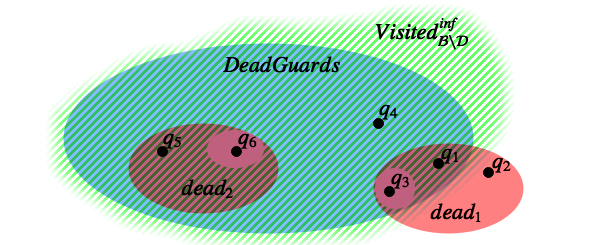
\includegraphics[width=0.7\textwidth]{guarded-systems/img/conj-deadlocks-venn.png}
\captionsetup{singlelinecheck=off}
\caption[fig:conj-deadlocks-venn]{%
Venn diagram for sets $DeadGuards$, $\deadOne$, $\deadTwo$, $\visInf{\mB\smi\mD}{x}$:
\begin{itemize}
\item[($q_1$)] $\deadOne \cap DeadGuards \cap \visInf{\mB\smi\mD}{x} \neq \emptyset$ is possible:
               in $x$, 
               there is a process deadlocked in state $q_1$,
               there is a non-deadlocked process that visits $q_1$ infinitely often,
               and there is a process deadlocked in a state $q \neq q_1$ 
               with a transition guarded ``$\forall \neg q_1$'' 

\item[($q_3$)] $\deadOne \cap DeadGuards \smi \visInf{\mB\smi\mD}{x} \neq \emptyset$ is possible:
               similarly to $q_1$, 
               except that no non-deadlocked processes visit $q_3$ infinitely often

\item[($q_2$)] $\deadOne \smi (\visInf{\mB\smi\mD}{x} \cup DeadGuards) \neq \emptyset$ is possible:
               in $x$, 
               there is a process deadlocked in state $q_2$,
               no other processes visit $q_2$ infinitely often,
               and no processes are deadlocked with a transition guarded ``$\forall \neg q_2$''

\item[($q_4$)] $DeadGuards \smi \dead \neq \emptyset$ is possible:
               there is a process deadlocked in a state $q \neq q_4$ 
               with a transition guarded  ``$\forall \neg q_4$''

\item[($q_5$)] $\deadTwo \cap \visInf{\mB\smi\mD}{x} \cap DeadGuards \neq \emptyset$ is possible:
               there is at least one process deadlocked in $q_5$ with a transition guarded ``$\forall \neg q_5$'',
               and some non-deadlocked process visits $q_5$ infinitely often
               (this process does not deadlock in $q_5$, 
                because in $q_5$ it receives an input different from that of the deadlocked processes)

\item[($q_6$)] $\deadTwo \cap DeadGuards \smi \visInf{\mB\smi\mD}{x} \neq \emptyset$ is possible:
               similarly to $q_5$, except no non-deadlocked processes visit $q_6$ infinitely often
\end{itemize}
}
\label{fig:conj-deadlocks-venn}
\end{mdframed}
\end{figure}

Let us assume $DeadGuards \neq \emptyset$---the other case is straightforward.\ak{check}

The construction has two phases, the setup and the looping phase.

In the {\bf setup phase}, we copy from $x$ into $y$:
\li
\-[a.] $y(A) = x(A)$;

\-[b.] for every $q \in \deadOne$: 
   devote one process of \cutoffsys that copies 
   a process of \largesys deadlocked in $q$;

\-[c.] for every $q \in \deadTwo \setminus \visInf{\mB\smi\mD}{x}$: 
   devote two processes of \cutoffsys that copy 
   the behaviour of two processes of \largesys that deadlock in $q$;

\-[d.] for every $q \in \deadTwo \cap \visInf{\mB\smi\mD}{x}$:
   in $x$, 
   there is a process, $B_q^\inf \in \mB\smi\mD$, that visits $q$ infinitely often,
   and there is a process, $B_q^\bot \in \deadTwo$, deadlocked in $q$.
   Then:
\li
   \-[1.] devote one process of \cutoffsys that copies the behaviour of $B_q^\bot$, and
   \-[2.] devote one process of \cutoffsys that copies the behaviour of $B_q^\inf$ 
          until it reaches $q$ at a moment after $d$,
          and then provide the same input as $B_q^\bot$ receives at moment $d$.
          This will deadlock the process;
\il

\-[e.] for every $q \in DeadGuards \setminus \dead$:
       note that $q \in \visInf{\mB\smi\mD}{x}$ and, thus, there is a process, 
       $B_q^\inf \in \mB\smi\mD$, 
       that visits $q$ infinitely often.
       Devote one process of \cutoffsys that copies the behaviour of $B_q^\inf$ 
       until it reaches $q$ at a moment after $d$;

\-[f.] if $DeadGuards \setminus \dead \neq \emptyset$ 
       or $A \in \mD$,
       then devote one process that stays in $\init_B$.
       The process will be used in the looping phase to ensure that the run $y$ is infinite,
       and that every process of \cutoffsys used in (e) 
       moves infinitely often (and thus $y$ is strong-fair);
       and
%       Note that if $A$ moves infinitely often in $x$ and $DeadGuards \smi \dead = \emptyset$,
%       then there is no need for such additional infinitely moving process.

\-[g.] let any other process of \cutoffsys (if any) 
       copy behaviour of a process of \largesys 
       that was not used in the construction so far (including this step).
\il
\ak{go through every item, and prove it is necessary (by giving an example)}
The setup phase ensures: 
in every state $q \in \dead$,
there is at least one process deadlocked in $q$ at moment $d$ in $y$. 
Now we need to ensure that the non-deadlocked processes described 
in steps (e) and (f) move infinitely often,
which is done using the looping extension described bellow.

The looping phase is applied to processes in (e) and (f) only\footnote%
{%
  If there are no such processes, then the setup phase produces the sought run $y$.
}.

Order arbitrarily 
$DeadGuards \smi \dead = (q_1,\ldots,q_k) \subseteq \visInf{\mB\smi\mD}{x}$.
Note that $\init_B \not\in (q_1,...,q_k)$.
Let $\mP$ be the set of processes of \cutoffsys used in steps (e) or (f).
Note that $|\mP| = |(q_1,...,q_k)| + 1$.

The \textbf{looping phase} is:
set $i=1$, and repeat infinitely the following.
\li
  \- Let $P_\init \in \mP$ be the process that is currently in $\init_B$, 
     and $P_{q_i} \in \mP$ -- in $q_i$.
     
  \- Let $B_{q_i} \in \visInf{\mB\smi\mD}{x}$ be a process of \largesys 
     that visits $q_i$ and $\init_B$ infinitely often.
     Let $P_\init$ of \cutoffsys copy transitions of $B_{q_i}$
     on some path $\init_B \to \ldots \to g_i$,
     then let $P_{g_i}$ copy transitions of $B_{q_i}$ on some path 
     $g_i \to \ldots \to \init_B$. 
     For copying we consider only the paths of $B_{q_i}$ that happen after moment $d$.

  \- $i=i \oplus 1$.
\il

The number of copies of $B$ that the construction uses in the worst case is 
(i.e., the item (g) is not used, and we assume $Q_B>2$, $DeadGuards \smi \dead = \emptyset$, and $A \in \mD$):
$$
1_{(f)} + 2|\deadTwo|_{(c),(d)} + |\deadOne|_{(b)} 
 \leq 
2|Q_B \smi \{\init_B\}| + 1.
$$

\myparagraph{Deadlocks}
The largest value of $c$ among those for ``Local Deadlocks'' 
and for ``Global Deadlocks'' can be used as the sought value of $c$ 
for the case of general deadlocks.
But it will not be the smallest one.
In the proof of the case ``Local Deadlocks'', in the setup phase, 
item (e) can be modified for the case when $A \in \mD$:
since we do not need to ensure that $y$ is infinite, 
we avoid allocating a process in state $\init_B$.
For a given locally deadlocked strong-fair run, the setup phase may produce
the globally deadlocked run, but that is allright for the case of general deadlocks.
With this note, for the general case $c = 2|Q_B \smi \{\init_B\}|$.
%
%\li
%  \-[a.] $y(A^1) = x(A^1)$
%  \-[b.] for each $q \in \deadOne(x)$: devote one process of \cutoffsys that mimics a process of \largesys that deadlocks in $q$\ak{replace `mimic' -- copy?}
%
%  \-[c1.] for each $q \in \deadTwo(x) \smi BlockStates$: devote two processes of \cutoffsys that mimic two processes of \largesys that deadlock in $q$
%  \-[c2.] for each $q \in \deadTwo(x) \cap BlockStates$: devote one processes of \cutoffsys that mimic one processes of \largesys that deadlocks in $q$
%  \-[d.] for each $q \in BlockStates$ devote one process of \cutoffsys that mimics a process $p_q$ that is in state $q$ at moment $d$. Note that such process in \largesys exists. 
%  
%  \-[e.] if $BlockStates \neq \emptyset$, then devote one process of \cutoffsys that stays in $\init$
%
%%   \-[d2.] Note \largesys has a process $p_q'$ different from $p_q$ from (d1) that enters $q$ infinitely often. Process $p_q'$ also visits $\init$ infinitely often. Thus, devote one process of \cutoffsys that stays in $\init$. Let $m_{qq}$ be some moment after 
%%   \li
%%     \-[d1.] if there is a process in \largesys that loops $q\to q$ infinitely often, then devote one process of \cutoffsys that mimics this process
%
%%     \- every process of \largesys that enters $q$ later exits $q$. Hence there are two processes of \largesys that meet in $q$ at some moment $m_{qq}$: devote two processes $p_1,p_2$ of \cutoffsys that mimic the behaviour of such processes till they meet in $q$ at the moment $m_{qq}$.
%%     Now observe that there is an infinite number of looping paths from $q \to \ldots\to q$ in the run $x$ by processes that enter $q$ and exit $q$ infinitely often.
%%     Starting from moment $m_{qq}$ interleave loopings between processes $p_1,p_2$, namely, start with $p_1$: stutter them both until some process of \largesys does the looping $q\to \ldots \to q$, and let process $p_1$ repeat that looping while keeping process $p_2$ in $q$.
%%     Now change turns: stutter them both until the moment when some process of \largesys does the looping $q \to \ldots \to q$, and let $p_2$ repeat the looping while keeping $p_1$ in state $q$. And so on.\ak{needs formalization}
%%   \il 
%
%  \-[f.] let any other process of \cutoffsys (if any) mimic a process of \largesys that was not used in the construction so far (including step (e))
%\il
%The setup phase ensures that in every state in $\dead(x)$ there is at least one process deadlocked at moment $d$ in $y$. Now we need to ensure that non-deadlocked processes described in step (d) move infinitely often.
%
%The looping phase applies to processes in (d) and (e) only. Order arbitrarily $BlockStates=(g1,\ldots,g_k)$. Then, set $i=1$, and repeat infinitely:
%\li
%  \- let $B^\init$ be the process from step (d) or (e) that is currently in $\init$, and $B^{g_i}$ is the one from (d) or (e) that is in $g_i$
%  \- in $x$ state $g_i$ is visited infinitely often by a process of \largesys that starts in $\init$. Hence, let $B^\init$ mimic that process on its loop from $\init \to \ldots\to g_i$, then let $B^{g_i}$ mimic that process on $g_i \to \ldots \to \init$
%  \- $i=i \oplus 1$
%\il
%The construction uses (if ignore (f)) assuming $Q_B>2$ and in the worst case (when $BlockStates$ is empty) $|\deadOne(x)| + 2|\deadTwo(x)| \leq 2|Q_B\smi \{ \init \}|$ processes B.
%
% The upper bound on the number of processes used in the construction of $y$ is $2(|BlockSet|-1) \leq 2|B|-2$.
%
% \input{other/disjoint-conj-dead-fair-proof-trial}
\end{proof}


\begin{tightness}[1-Conj, Deadlocks, Fair] \label{obs:conj:tight_deadlock_fair}
The cutoff $c=2|B|-2$ is tight for deadlock detection on strong-fair initializing
or finite runs in the 1-conjunctive systems, 
i.e., 
for any $k>2$ there is a system type $(A,B)$ with $|B|=k$ such that 
there is a strong-fair initializing deadlocked run in $(A,B)^{(1,2|B|-2)}$, 
but not in $(A,B)^{(1,2|B|-3)}$.
\end{tightness} 
\begin{proof} 
Consider the same templates as in Tightness~\ref{obs:conj:tight_deadlock}.
%
% AK: we can claim the below, but we need to note that 
% the monotonicity lemma for local deadlocks also holds (straightforward)
% let's comment this out for now.
%  Note that the cutoff $c=2|B|-1$ stated in the previous Lemma 
% for the case of local deadlocks is also tight.
% To prove this, take the templates from Observation~\ref{obs:conj:tight_deadlock}
% and modify slightly the template B:
% add the unguarded self-loop to $\init$.
%%%
% \begin{figure}[Htb]
% \centering
% \subfloat[Template A]{
% \centering
% \makebox[0.4\textwidth][c]{
% \scalebox{0.75}{% !TEX root = table.tex
\begin{tikzpicture}[node distance=2.3cm,inner sep=1pt,minimum size=0.5mm,->,>=latex]


\node[initial left, state] (init) {};

\path (init) [loop right] edge [right] node {$\forall\neg 1_B$} (init);
\path (init) [loop right,dotted,distance=26mm] edge [right] node {...} (init);
\path (init) [loop right,distance=38mm] edge [right] node {$\forall\neg k_B$} (init);


\end{tikzpicture}
  
}
% \label{fig:conj:tight_deadlock_tmplA}
% }}
% \subfloat[Template B]{
% \centering
% \makebox[0.6\textwidth][c]{
% \scalebox{0.75}{% !TEX root = table.tex
\begin{tikzpicture}[node distance=2.4cm,inner sep=1pt,minimum size=0.5mm,->,>=latex]


\node[initial above, state] (init) {$init$};
\node[state] (b_1) [left=2.7cm of init] {$1_B$};
\node (dots) [below=1cm of init] {$\ldots$};
\node[state] (b_k) [right=2.7cm of init] {$k_B$}; 

% \path (b_1.20) edge [above] node {\specialcell{$\forall{\neg b_1}$\\...\\$\forall{\neg b_k}$}} (init.160);
\path (b_1.20) edge [above] node {$\forall{\neg 1_B},...,\forall{\neg k_B}$} (init.160);
\path (init.200) edge [above] node {} (b_1.340);

\path (b_k.160) edge [above] node {$\forall{\neg 1_B},...,\forall{\neg k_B}$} (init.20); 
\path (init.340) edge [above] node {} (b_k.200); 

\path (init.282) edge [left, dotted] node {} ($(dots)+(0.1,0.1)$);
\path ($(dots)-(0.1,-0.1)$) edge [left, dotted] node {$\forall{\neg 1_B},...,\forall{\neg k_B}$} (init.257);

% \path (b_1) [loop left] edge [left] node {$\forall\neg b_1$} (b_1);
% \path (b_1) [loop left,dotted,distance=26mm] edge [left] node {...} (b_1);
% \path (b_1) [loop left,distance=38mm] edge [left] node {$\forall\neg b_k$} (b_1);

% \path (b_k) [loop right] edge [right] node {$\forall\neg b_1$} (b_k);
% \path (b_k) [loop right,dotted,distance=26mm] edge [right] node {...} (b_k);
% \path (b_k) [loop right,distance=38mm] edge [right] node {$\forall\neg b_k$} (b_k);


\end{tikzpicture}
  
}
% \label{fig:conj:tight_deadlock_tmplB}
% }}
% \caption{Templates $(A,B)$ used to prove the tightness of the cutoff $c=2|B|-2$ for the deadlock detection in 1-guard conjunctive systems.
% In the figure the edge with $\forall{\neg b_1},\ldots,\forall{\neg b_k}$ denotes edges with guards $\forall{\neg b_1},\ldots,\forall{\neg b_k}$ (Observation~\ref{obs:conj:tight_deadlock}).\ak{check me}}
% \label{fig:conj:tight_dead_tmpl}
% \end{figure}
\end{proof}


%\section{Experiments} \label{gua:sec:experiments}

(The experiments were done by S. Au{\ss}erlechner,
 as a part of his Master Thesis.)

We used our new cutoff results in the context of parameterized synthesis to 
automatically construct process templates with safety and liveness guarantees 
for guarded systems with an arbitrary number of components.
Our prototype is an extension of the parameterized synthesis tool 
{\sc Party}~\cite{party}.
It synthesizes process templates based on the semi-decision procedure 
described in Section~\ref{gua:sec:paramsynt}. 
Bounded template synthesis is 
implemented as an extension of the bounded synthesis approach~\cite{BS}, with
LTL3BA~\cite{LTL3BA} for translation of specifications to automata, and
SMT solver Z3~\cite{Moura08} as backend. 

%In the cutoff detection step, we apply the cutoff results from 
%Section~\ref{gua:sec:cutoffs} modularly, i.e., we calculate cutoffs and convert 
%to universal co-Büchi tree automaton (UCT)\sj{remind/use long version} for every conjunct of the specification separately (an optimization 
%mentioned in~\cite{KhalimovJB13b}). Finally, we produce the SMT encoding, 
%conjoining the SMT constraints for all parts. 
%
As a proof of concept, we synthesized implementations for two small 
examples (on a single core of a 3.5GHz Intel i7 CPU with 4GB RAM):
\begin{itemize}
\item a closed disjunctive system $\largesys$ where $A$ controls an output 
signal $w$, and every $B_i$ a signal $g_i$, with fairness assumption and specification
$\GF(\neg w) \wedge \GF w \wedge 
\bigwedge_{i} \left[\GF(w \wedge g_i) \wedge  \GF g_i \wedge \GF(\neg g_i) 
\right]$,
i.e., all processes must toggle their signals 
infinitely often, and every process $B^i$ must ``meet'' infinitely often with 
$A$ when both signals are enabled. The implementation below has been synthesized with a cutoff of $2\card{B}+1-1=4$ for the property and $2\card{B}-1=3$ for the deadlock detection within one minute.

\item an open conjunctive system $(B)^{(n)}$ (i.e., $A$ can be arbitrary and $B$ does not react to it), where each process $B_i$ gets requests of high and low priority as input ($rh_i, rl_i$), and controls ouputs that represent grants to these requests ($gh_i, gl_i$). The specification requires i) `every request $rh$ should eventually be granted ($gh_i$)', ii) `every request $rl_i$ should eventually be granted ($gl_i$) unless there is a simultaneous request $rh_i$', iii) `there should be no spurious grants', iv) `mutual exclusion of grants (locally and globally)'. The implementation above has been synthesized with a cutoff of $3$ for properties, and $4$ for deadlock detection within about $45$ minutes. Note that we do not restrict the implementation to $1$-conjunctive systems, and therefore the cutoff does not guarantee absence of local deadlocks in systems of arbitrary size.
\end{itemize}

\begin{figure}[ptb]
\centering
\begin{subfigure}[b]{0.45\textwidth}\center
\scalebox{0.7}{\begin{tikzpicture}[->,>=stealth',shorten >=1pt,auto,node distance=1.6cm,
                    semithick]
  \tikzstyle{every state}=[align=center,anchor=center]
  \tikzstyle{every edge} = [align=center,draw=black]
  \tikzstyle{boxLabel} = [yshift=-0.4cm]
  \tikzstyle{box} = [draw=black, inner sep=0.75cm]
	
  \node[state] (t00) [label={left:$\neg w$}]                    {$0_A$};
  \node[state] (t01) [below of=t00,label={left:$w$}] {$1_A$};
  \coordinate (t00') at ($(t00.west) + (-1.0cm,0.5cm)$);
  \coordinate (t01') at ($(t01.east) + (+0.75cm,-0.25cm)$);
  \node (U1) [draw=black, fit=(t00') (t01'), inner sep=0.75cm] {} ;
  \node [boxLabel] at (U1.north) {Template $A$};
  
  \path (t00) edge [bend right,left] node {$\exists \left\{0_B, 1_B\right\}$} (t01)
            (t01) edge [bend right, right] node {$\exists \left\{1_B\right\}$} (t00);

   
   
  \node[state] (t10) [label={left:$\neg g$},right of=t00,node distance=4.5cm] {$0_B$};
  \node[state] (t11) [label={left:$g$}, below of=t10] {$1_B$};
  \coordinate (t10') at ($(t10.west) + (-0.75cm,0.5cm)$);
  \coordinate (t11') at ($(t11.east) + (+0.75cm,-0.25cm)$);
  \node (U2) [box,fit=(t10') (t11')] {} ;
  \node [boxLabel] at (U2.north) {Template $B$};
  
  \path (t10) edge [bend right,left] node {$\exists \left\{1_A\right\}$} (t11)
            (t11) edge [bend right, right] node {$\exists \left\{1_A\right\}$} (t10);
  %\draw[ltsBox,label={above:x},anchor=center] ($(t10.north west)+(-1.7,0.6)$)  rectangle ($(t11.south east)+(1.7,-0.6)$); 
\end{tikzpicture}
}
\caption{Disjunctive system}
\label{fig:disjunctiveLTS}
\end{subfigure}
\begin{subfigure}[b]{0.45\textwidth}\center
\scalebox{0.7}{\begin{tikzpicture}[->,>=stealth',shorten >=1pt,auto,node distance=1.5cm,
                    semithick]
  \tikzstyle{every state}=[align=center, anchor=center]
  \tikzstyle{every edge} = [align=center,draw=black,]

  \node[state] (A) [label={below:$$}] {$0_A$};
  \node[] (BC) [below of=A] {$$};
  \node[state] (B) [left of=BC, label={below:$gh$}] {$1_A$};
  \node[state] (C) [right of=BC, label={below:$gl$},] {$2_A$};


  \path 
  (A) edge [loop above] node {$\neg rh \wedge \neg rl : \forall \{0_A\}$} (A)
  (A) edge [left, bend right=10] node {$rh: \forall \{0_A\}$} (B)
  (B) edge [right, pos=0.3, bend right=10] node {$*: \forall \{0_A\}$} (A)
  (A) edge [right, bend left=10] node {$\neg rh \wedge rl: \forall \{0_A\}$} (C)
  (C) edge [right, bend left=10] node {$$} (A);
\end{tikzpicture}}
\label{fig:conjunctiveLTS3}
% \caption{Templates $(A,B)$ used to prove the tightness of the cutoffs for properties $\pexists h(A^1,B^1)$ (Observation~\ref{obs:disj:tight_prop})\ak{check me}.}
\label{fig:experiments}
\caption{Conjunctive system}
\end{subfigure}
\caption{Synthesized systems}
\end{figure}

\section{Conclusion} \label{gua:sec:concl}

We have extended the cutoffs for guarded protocols of Emerson and 
Kahlon~\cite{Emerson00} to support local deadlock detection, fairness 
assumptions, and open systems.
In particular, our results imply the decidability of the parameterized model checking problem for this class of systems and specifications,
which to the best of our knowledge was unknown before. 
%Our results allow us to model check
%guarded protocols that satisfy not 
%only safety, but also liveness conditions, for an arbitrary number of 
%components. 
Furthermore, the cutoff results can easily be integrated into 
the parameterized synthesis approach~\cite{JB14}.
%~\cite{Jacobs14,Khalimov13,Khalimov13a}.

%An approach for using cutoff results in 
%synthesis has been introduced by 
%Jacobs and Bloem~\cite{Jacobs14}. It has been described in detail for the 
%case of 
%token-passing systems. Follow-up papers have shown how to make the approach 
%more efficient~\cite{KhalimovJB13b}, and how to use it for the synthesis of a 
%large 
%case study, the AMBA bus arbiter~\cite{BloemJK14}.

Since conjunctive guards can model atomic sections and read-write locks, 
and disjunctive guards can model pairwise rendezvous 
(for some classes of specifications, see~\cite{EmersonK03}), 
our results apply to a wide spectrum of systems models.
But the expressive power of the model %and flexibility of the results 
comes at a high cost: cutoffs are linear in the size of a process, and 
are shown to be tight (with respect to this parameter).
For conjunctive systems, our new results are restricted to systems with
1-conjunctive guards, effectively only allowing to model a single shared
resource. 
We conjecture that our proof methods can be extended to systems with
more general conjunctive guards, at the price of bigger cutoffs.
We leave this extension and the question of finding cutoffs that are independent of the size of processes for future research.

We did preliminary experiments~\cite{SimonThesis} by implementing the synthesizer inside our parameterized synthesizer PARTY~\cite{party}.
It is a possible future work to find and apply it to real-world applications.
%
%
%We are working on a prototype implementation (\url{https://bitbucket.org/parsy/guarded_synthesis/}), which however is currently limited to very small systems.\sj{we should re-formulate or remove the comment on implementation} 
%In future work, we will try to lift the restrictions of our results for conjunctive systems, and investigate cutoffs that are independent of the size of the components' state spaces.
%\ak{remove this promise?}
\ak{note that EK have better complexities for 'for all paths' properties. 
As a future work, one can look if our cutoffs can be improved.}
%This is due 
%to the growth of the cutoff (linearly) and the set of possible transition 
%guards (doubly exponential) in the size of process templates. 
%In the future, 
%we will look into cutoffs that are independent of the size of process 
%templates.

